% paper.tex  ---  Gas Reservoirs Predict Future Galaxy Growth Beyond Halo Assembly History in CAMELS (TNG/SIMBA)
% Compile: ./build.sh  (runs paper.py then latexmk)
% Requires outputs/ generated by paper.py
% Format: AASTeX 7.0.1  (aastex701.cls)

\documentclass[twocolumn,linenumbers]{aastex701}

\usepackage{booktabs}
\usepackage{multirow}
\usepackage{float}
\usepackage{microtype}
\usepackage{enumitem}

% ---- Macros generated by paper.py ------------------------------------------
% paper_macros.tex  ---  numeric macros used by paper.tex
%
% PROVENANCE.  This file is NOT fully regenerated by build.sh.  build.sh runs
% paper.py, whose _write_macros() emits only the core whole-sample macros; the
% values below are the manuscript-facing subset, each RECORDED from a named,
% tracked computed output and independently verified against it (see the audit
% trail in outputs/referee/ and referee_scripts/).  To update a value, re-run
% the cited analysis and copy the number here; do not edit by guesswork.
%
% Only macros actually referenced by paper.tex are kept (stale/unused macros
% were removed).  Every value here has been checked to match its source file.

% ---- Sample sizes (matched catalogs) ---------------------------------------
% TNG: SubLink-matched; SIMBA: spatially matched. Mid/low/high partition the
% TNG SubLink sample at logM* = 9.55 and 10.55 (2,902 + 3,430 + 1,030 = 7,362).
\newcommand{\TNGSubLinkN}{7{,}362}
\newcommand{\SIMBASpatialN}{4{,}203}
\newcommand{\MidMassN}{3{,}430}
\newcommand{\LowMassN}{2{,}902}
\newcommand{\HighMassN}{1{,}030}

% ---- Sliding-window scan  (outputs/baseline_B/results_mass_scan_l3.json) ----
% WindowNWindowsL = # windows with L3 internal marginal CI>0 (9.55-10.55);
% WindowPeakMarg = max L3 internal marginal (at centre 10.35).
\newcommand{\WindowLoL}{9.55}
\newcommand{\WindowHiL}{10.55}
\newcommand{\WindowNWindowsL}{11}
\newcommand{\WindowPeakMarg}{0.161}

% ---- Paired gap internal-halo under L3
%      (outputs/baseline_B/results_mass_scan_l3_quench_pg.json, paired_L3) -----
% NWindows = # windows with delta CI>0; Lo/Hi = min/max delta over 9.55-10.55.
\newcommand{\PairedGapNWindows}{13}
\newcommand{\PairedGapLo}{+0.052}
\newcommand{\PairedGapHi}{+0.089}

% ---- f_star / L3 absorption  (outputs/referee/fstar_absorption_summary.csv) -
\newcommand{\FstarInternalMarg}{0.086}
\newcommand{\FstarInternalCILo}{+0.043}
\newcommand{\FstarInternalCIHi}{+0.133}
\newcommand{\FstarHaloMarg}{0.017}
\newcommand{\LThreeInternalMarg}{0.135}
\newcommand{\LThreeHaloMarg}{0.083}

% ---- SIMBA L1 quenching peak (outputs/referee/simba_same_control_scores.csv)-
\newcommand{\SimbaQuenchPeak}{0.141}

% ---- Mid-mass raw family scores
%      (outputs/baseline_B/results_geoctrl_l2.json, delta_logmstar) -----------
\newcommand{\MidMassInternalR}{0.307}
\newcommand{\MidMassHaloR}{0.235}
\newcommand{\MidMassGap}{+0.072}

% ---- Spatial-vs-SubLink matching confound
%      (L1 internal baseline: baseline_A spatial vs baseline_B SubLink) -------
% SpatialInflation = SpatialBaselineTNG / SubLinkBaseline.
\newcommand{\SpatialInflation}{3.7}
\newcommand{\SubLinkBaseline}{0.059}
\newcommand{\SpatialBaselineTNG}{0.220}
\newcommand{\SpatialBaselineSIMBA}{0.273}

% ---- Assembly ablation
%      (outputs/referee/unresolved_absorption_feature_groups.csv;
%       outputs/baseline_B/results_geoctrl_l3_9p5_10p5_geomabl_*.json) --------
% Recovery = (ablated internal marginal) - (full-L3 internal marginal).
% Timing recovery is the source value 0.0253 (-> +0.025), not 0.161-0.135.
% Pct = recovery as a fraction of the published L3 decomposition.
\newcommand{\AblationTimingRecovery}{+0.025}
\newcommand{\AblationTimingPct}{19}
\newcommand{\AblationLongAccretionRecovery}{+0.014}
\newcommand{\AblationLongAccretionPct}{10}
\newcommand{\AblationMergerRecovery}{+0.000}


% ---- Paper-level shorthand macros ------------------------------------------
\newcommand{\logM}{\log M_*}
\newcommand{\Rmarg}{R^2_\mathrm{marg}}
\newcommand{\Rgeom}{R^2_\mathrm{geom}}
\newcommand{\fstar}{f_*}
\newcommand{\dlogM}{\Delta\!\logM}

\begin{document}

\title{Gas Reservoirs Predict Future Galaxy Growth Beyond Halo Assembly
       History in CAMELS}

% Double-blind placeholder
\author{Anonymous}
\affiliation{Affiliation withheld for review}
\email{placeholder@placeholder.com}

% ---------------------------------------------------------------------------
\begin{abstract}
Does a galaxy's gas content tell us anything about its future growth once its
dark-matter halo history is already known? We test this question in the CAMELS
CV suite using 27 fixed-parameter realizations of the IllustrisTNG and SIMBA
galaxy-formation models. For each galaxy, we compare three predictor families
--- internal galaxy properties, halo/assembly-history properties, and
environment --- as predictors of future stellar growth, quenching, and halo
growth from $z \simeq 0.77$ to $z = 0$. We measure how much predictive power
each family adds beyond increasingly strict halo controls, ending with a
13-feature assembly-history baseline.

In TNG, gas reservoir information predicts future stellar growth beyond the
full assembly-history control at low-to-intermediate stellar mass, up to
$\logM/M_\odot \simeq 10.55$. This is not simply a current-star-formation
effect: the gas signal survives controls for stellar mass, SFR, and sSFR. It
is also not a gas-use-efficiency effect: gas amount remains informative, while
depletion time adds no comparable information once gas amount is included.
Halo assembly history strongly predicts the gas reservoir itself
($R^2 \simeq 0.8$), but the residual gas component still predicts future
growth. Thus the gas reservoir is shaped by halo history but not exhausted by
it.

Near $\logM/M_\odot \simeq 10.55$, the predictive structure changes.
Black-hole/quenching state, traced by catalog-level black-hole proxies rather
than direct feedback-energy measurements, becomes more informative, and the
high-mass population is largely quenched. The full assembly-history (L3) control is available only for TNG; because
SubLink-equivalent merger trees are unavailable for SIMBA, we compare the two
models at a matched static-halo (L1) control, where they express residual
baryonic information in different channels --- stellar growth in TNG and
quenching in SIMBA --- with no SIMBA L3-controlled claim. We caution that the low-mass edge is
resolution/floor-sensitive rather than a sharp physical threshold, and that the
environment result is limited to the CAMELS CV volume and features. Overall,
the results support a fuel-limited to quenching-limited picture of future
galaxy growth and motivate an observational test: gas-rich galaxies should
grow preferentially at fixed stellar mass and assembly proxies in surveys such
as xGASS\,/\,xCOLD\,GASS.
\end{abstract}

\keywords{galaxies: evolution --- galaxies: statistics ---
          methods: statistical --- dark matter haloes ---
          galaxies: star formation --- galaxies: quenching}

% ---------------------------------------------------------------------------
\section{\textbf{Introduction}}
\label{sec:intro}

A central question in galaxy formation is which properties best predict how
a galaxy will grow or quench over the coming few gigayears.
Three families of properties are routinely discussed: the internal baryonic
state of the galaxy (gas content, star-formation rate, stellar mass), the
properties of its host dark matter halo (mass, concentration, spin,
formation history), and the large-scale environment (local density, group
richness, filamentary structure).
A substantial literature has addressed each family in isolation
\citep[e.g.,][]{dave2012,wetzel2013,behroozi2019,moster2013,peng2010},
and a growing body of work connects galaxies to their dark matter halos
across cosmic time \citep{wechsler2018,gao2005,wechsler2006,mao2018},
but systematic comparisons under the same sample, time horizon, and
control structure are less common.

The difficulty is that these families are not independent.
Halo mass correlates with environment.
Gas content correlates with halo assembly history through the rate at which
gas is accreted --- via cold streams at high redshift and hot-halo cooling
at later times \citep{dekel2009} --- and feedback-driven outflows are
recycled \citep{bouche2010,lilly2013}.
Stellar mass --- part of any internal description --- is itself a record of
past growth, and therefore implicitly encodes assembly history.
Correlations between a property family and a future outcome can therefore
reflect the gravitational context rather than baryonic processes specific to
that family.
The standard approach of correlating present-day properties with future
states --- whether via classical statistics or machine-learning feature
ranking \citep[e.g.,][]{bluck2022,davies2019,teimoorinia2016,lovell2019,matthee2019}
--- does not cleanly separate these contributions.

A sharper question is: after controlling for what the halo structural and
assembly history already predicts, does a galaxy's internal baryonic state
carry additional information about its future?
And does the answer depend on stellar mass?
Several results suggest it might.
Observations and simulations show that galaxy growth at intermediate stellar
mass ($\logM \sim 9.5$--$10.5$) is particularly sensitive to gas supply
and feedback \citep{dave2012,pillepich2018gas,saintonge2017}, while at low
mass, growth tracks the large-scale structure and tidal field, and at high
mass, AGN feedback and the halo potential increasingly dominate quenching
\citep{croton2006,weinberger2018,peng2010}.
If the coupling between baryonic state and future growth is genuinely
mass-regime-specific, then a global comparison of predictor families will
miss the structure.

We address this directly using the CAMELS Cosmic Variance (CV) suite
\citep{villaescuza-navarro2021}, which provides 27 independent realizations
each of IllustrisTNG \citep{weinberger2017,pillepich2018} and SIMBA
\citep{dave2019} at fixed astrophysical parameters.
The statistical independence of the 27 realizations allows bootstrap
confidence intervals on predictive scores to be evaluated at population
level rather than for individual realizations.
We construct three predictor families from early-epoch ($z \approx 0.77$)
galaxy properties and ask how well each predicts three outcomes at $z = 0$
(stellar growth, quenching, and halo growth), both in the whole sample and
as a function of stellar mass.
The central diagnostic is a marginal score: the increment in
cross-validated predictive performance when a feature family is added to a
halo assembly-history control, evaluated by shared bootstrap.
This directly measures whether a feature family carries predictive
information beyond the halo's gravitational record.

The key developments are as follows.
No feature family leads consistently across all targets and mass regimes:
the $3 \times 3$ performance matrix shows statistical ties in both
simulation families.
Spatial matching inflates the assembly-history baseline \SpatialInflation$\times$
relative to merger-tree matching, a confound that must be accounted for
before cross-family assembly-control comparisons.
At low-to-intermediate stellar mass --- up to $\logM/M_\odot \simeq 10.55$ ---
internal gas-reservoir information retains predictive power for future stellar
growth beyond the full 13-feature assembly-history control.
This residual is carried by the gas \emph{amount}: it survives controls for
stellar mass and for the current (specific) star-formation rate, and it is not
a gas-use-efficiency (depletion-time) effect.
The reservoir is itself strongly predicted by halo assembly history, yet a
residual gas component continues to predict growth --- so the gas reservoir is
shaped by halo assembly history but not exhausted by it.
Near $\logM/M_\odot \simeq 10.55$ the predictive structure changes:
black-hole and quenching state --- traced by catalog-level black-hole proxies
rather than direct feedback-energy measurements --- becomes the more
informative channel, and the high-mass population is largely quenched.
The full L3 assembly-history control is available only for TNG; because
SubLink-equivalent merger trees are unavailable for SIMBA, we compare the two
feedback models at a matched static-halo (L1) control, where they express this
residual baryonic information in different channels --- stellar growth in TNG and
quenching in SIMBA --- and we make no SIMBA L3-controlled claim.
The lower edge of this regime is set by resolution and catalog-floor effects
rather than a sharp physical threshold; results are otherwise stable across all
27 CAMELS CV realizations and to the choice of halo structural variable.

% ---------------------------------------------------------------------------
\section{\textbf{Data and Methods}}
\label{sec:methods}

\subsection{CAMELS CV Suite}
\label{sec:data}

We use the Cosmic Variance (CV) sub-suite of CAMELS, comprising 27
independent realizations each of IllustrisTNG and SIMBA at fixed
cosmological and astrophysical parameters \citep{villaescuza-navarro2021}.
Each box is $25\, h^{-1}\,\mathrm{Mpc}$ with $256^3$ dark matter particles;
we use snapshots 066 and 090 ($z = 0.7747$ and $z = 0$).
We restrict to \textit{central} galaxies with $\logM(z=0.77) \geq 9.0$;
after matching the TNG SubLink sample contains $n = \TNGSubLinkN$ galaxies
and the SIMBA spatial sample $n = \SIMBASpatialN$.

\subsection{Predictor Feature Families}
\label{sec:features}

We define three predictor families, each evaluated independently using only
features from within that family.

\begin{deluxetable}{llll}
\tablecaption{Predictor feature families.\label{tab:features}}
\tablehead{
  \colhead{Family} & \colhead{$N_\mathrm{feat}$} &
  \colhead{Features} & \colhead{Source}
}
\startdata
Environmental & 4 &
  $\log M_\mathrm{halo}$, $\log N_\mathrm{subs}$,
  $\log \rho_\mathrm{local}$, $\log n_\mathrm{5Mpc}$ &
  FoF halo + neighbor count \\
Internal & 6 &
  $\log M_*$, $\log M_\mathrm{gas}$, $\log \mathrm{SFR}$,
  $\log \mathrm{sSFR}$, $\log R_*$, metallicity &
  Subhalo catalog \\
Halo structural & 5 &
  $\log M_\mathrm{sub}$, $V_\mathrm{max}$, $\log R_\mathrm{sub}$,
  spin, $V_\mathrm{max}/V_{200}$ &
  Subhalo + FoF \\
\enddata
\end{deluxetable}

All features are measured at the early epoch ($z = 0.77$).
The three families are evaluated independently so that their marginal
contributions can be assessed cleanly; no family has access to features of
any other family when scored.

\subsection{Targets}
\label{sec:targets}

Three outcomes are predicted at $z = 0$: stellar growth
($\dlogM = \logM(z=0) - \logM(z=0.77)$, Ridge $R^2$, 5-fold CV);
binary quenching ($\mathrm{sSFR}(z=0) < 10^{-11}\,\mathrm{yr}^{-1}$,
logistic Ridge AUC, 5-fold CV); and halo growth ($\Delta\log M_\mathrm{sub}$,
Ridge $R^2$).
Hyperparameters are tuned by inner cross-validation on the training fold.

\subsection{Matching Methods}
\label{sec:matching}

Tree-based SubLink matching \citep{rodriguez-gomez2015}, available for TNG
only, links each early-epoch galaxy to its $z=0$ descendant via merger trees,
introducing no structural selection bias; it is used for all assembly-history
control analyses.
Spatial matching --- nearest late-epoch galaxy within $3\times$ the
early-epoch half-mass radius --- preferentially selects structurally stable
systems, inflating the assembly-history baseline (Section~\ref{sec:confound}).
It is used for SIMBA, where SubLink-equivalent trees are unavailable.

\subsection{Significance Rule}
\label{sec:verdict}

A feature family is declared to lead over another if the bootstrap 95\% CI
lower bound of their score gap exceeds 0.02 ($R^2$ or AUC); otherwise the
result is declared a tie.
The threshold of 0.02 was fixed before interpretation and is not tuned to
produce a particular result.
It represents the minimum practically meaningful gap relative to the
observed bootstrap noise structure in the 27-simulation CV suite: gaps
below 0.02 are within the regime where small changes in simulation selection
or minor specification differences routinely flip the ordering sign, making
them uninformative as science claims.
The main results of this paper --- the upper-bounded intermediate-mass regime,
the flat paired gap, the carrier and ablation decompositions --- are
continuous statistics evaluated with 95\% bootstrap CIs and do not depend
on this threshold.
The TIE/WINNER declarations in
Sections~\ref{sec:whole_sample}--\ref{sec:mass_splits} do depend on it;
those conclusions are qualitatively stable to reasonable threshold
variation (at 0.01, the mid-mass growth WINNER verdict is unchanged; at
0.05, only the strongest gaps survive, but the mass-regime patterns are
preserved).

\subsection{Three-Layer Assembly-History Controls}
\label{sec:geometry}

To assess whether predictor family signals persist beyond what the halo
structural and assembly history already predicts, we apply a three-layer
control procedure to TNG SubLink.

L1 (static halo structure) uses three features describing where the halo
sits at $z = 0.77$: $\log M_\mathrm{halo}$, $\log \rho_\mathrm{local}$,
and $\log M_\mathrm{sub}$.
L2 augments L1 with $\Delta\log M_\mathrm{halo}$ over 4 and 8 SubLink steps
($\approx 1$--$2$ Gyr lookback) and halo formation snapshot.
L3 extends L2 with $\Delta\log M_\mathrm{halo}$ over 12 and 16 steps
($\approx 3$--$4$ Gyr lookback), peak mass ratio, half-mass assembly
snapshot, merger count, major-merger count (mass ratio $\geq 0.25$), and
last major-merger snapshot, for a total of 13 assembly-history features.

Three control statistics are computed for each predictor family.
The \textit{marginal} $R^2$/AUC is the increment in cross-validated score
when the family is added to the assembly-history control; 95\% CIs come from
a shared bootstrap ($n_\mathrm{boot} = 1000$).
\textit{Residualization} OLS-regresses each predictor feature column against
the assembly-history control set and replaces it with the OLS residual before
the predictive model is fit (it is the feature columns, not the target, that
are residualized).
\textit{Retention} is the ratio of residualized to original score, with the
AUC analog computed on the $(x - 0.5)$ excess.

\subsection{Robustness Tests}
\label{sec:robustness_design}

Two robustness checks are applied throughout:
\begin{enumerate}
  \item \textit{Simulation jackknife}: leave one of 27 CV realizations out;
    report the fraction $n_\mathrm{agree}/27$ that preserve the full-sample
    ordering.
  \item \textit{Permutation importance}: shuffle each feature column; measure
    the mean drop in CV $R^2$ over $n_\mathrm{boot} = 500$ draws.
\end{enumerate}

% ---------------------------------------------------------------------------
\section{\textbf{Results}}
\label{sec:results}

\subsection{No Feature Family Leads Consistently Across Targets}
\label{sec:whole_sample}

The full $3 \times 3$ score matrix is in Appendix~\ref{app:tables}
(Table~\ref{tab:whole_sample}).
In both TNG SubLink and SIMBA spatial, every cell is a tie: no feature
family leads across all three targets, and every pairwise gap has a 95\%
CI spanning or approaching zero.

\begin{figure*}[t!]
\centering
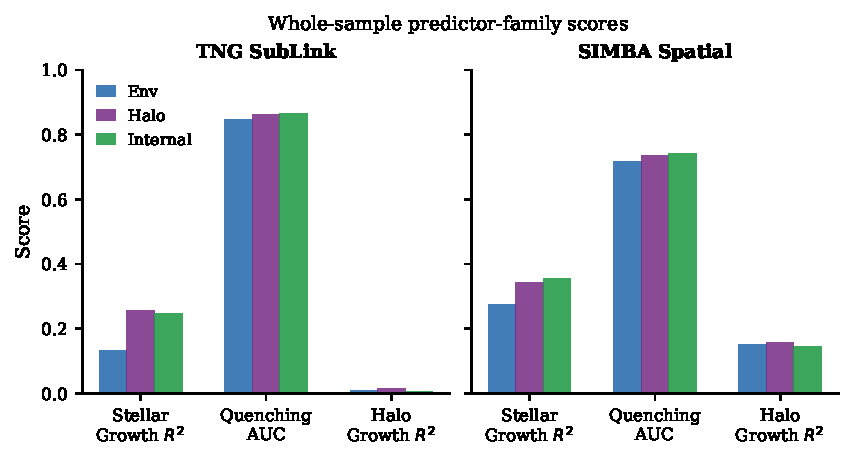
\includegraphics[width=\textwidth]{outputs/figures/fig01_score_matrix.pdf}
\caption{Full $3 \times 3$ score matrices for TNG SubLink (left) and SIMBA
  spatial (right).
  Color encodes class score ($R^2$ or AUC).
  All cells are statistical ties in both simulation families.
  The whole-sample tie is the surface pattern; the mass-regime structure
  revealed by sliding-window analysis is the main result
  (Figure~\ref{fig:phase_diagram}).
\label{fig:matrix}}
\end{figure*}

The tie is robust across both simulation families: TNG and SIMBA agree on
winner structure despite differing in overall predictability level.
Within-target ordering is target-dependent (growth favors internal at mid
mass; quenching favors internal in both), motivating the mass-regime
decomposition below.
Cross-family quantitative differences are partly a matching artifact
(Section~\ref{sec:confound}) and are not interpreted as clean physics signals.
Halo growth ($\Delta\log M_\mathrm{sub}$) is near-unpredictable by any family
at $z \approx 0.77$ ($R^2 \leq 0.015$ across all three families in TNG;
Table~\ref{tab:whole_sample}). This bound is for the whole-sample structural
families; even the richer 13-feature L3 assembly-history context predicts
whole-sample halo growth at only $R^2 \approx 0.029$, and in the intermediate
window every family remains $\lesssim 0.016$ (internal $+0.009$, halo $+0.016$,
environment $+0.000$) --- an order of magnitude below stellar growth, where the
internal family alone reaches $R^2 \sim 0.2$--$0.3$ in the same window. This
indicates that dark matter accretion between $z = 0.77$ and $z = 0$ is driven by
large-scale density fluctuations not encoded in the snapshot properties of
individual galaxies.
This contrast is itself informative: late dark-matter accretion is not well
encoded in individual $z \simeq 0.77$ subhalo, galaxy, or environment
properties in CAMELS CV, whereas baryonic stellar growth retains stronger
predictive structure --- a galaxy's baryonic future is more foreseeable than
its gravitational future at fixed epoch.

\subsection{Matching Method Confound}
\label{sec:confound}

The assembly-history baseline --- the $R^2$ achievable from static
structural position alone --- differs dramatically by matching method
(Table~\ref{tab:confound} in Appendix~\ref{app:tables}):
SubLink gives $R^2 = \SubLinkBaseline\,[0.051, 0.072]$; spatial matching
gives $R^2 = \SpatialBaselineTNG$ (TNG) and $R^2 = \SpatialBaselineSIMBA$
(SIMBA).

Spatial matching selects galaxies that remain structurally stable between
$z = 0.77$ and $z = 0$, inflating all predictor scores and the
assembly-history baseline \SpatialInflation$\times$.
The similarity between TNG spatial and SIMBA spatial baselines is partly a
matching artifact, not a physics signal.
\textbf{All assembly-history control analyses in this paper use TNG SubLink
exclusively.}
The mechanistic findings of Sections~\ref{sec:window}--\ref{sec:mechanism}
do not extend to SIMBA without SubLink-equivalent merger trees.

\subsection{Mass-Regime Splits: The Whole-Sample Tie is Misleading}
\label{sec:mass_splits}

The whole-sample tie conceals opposite orderings at different stellar masses
(Table~\ref{tab:mass_splits}, Appendix~\ref{app:tables}).
Mid mass ($9.5 \leq \logM < 10.5$) is the only regime with a clear growth
winner: internal $R^2 = \MidMassInternalR$ versus halo $= \MidMassHaloR$,
gap $= \MidMassGap$ (bootstrap 95\% CI lower bound $> 0.02$; see
Table~\ref{tab:gap} for the assembly-history-controlled lower bound,
$\PairedGapLo$--$\PairedGapHi$ across \PairedGapNWindows{} consecutive
windows).
At low mass, internal growth is near noise while environmental and halo
features lead; at high mass, the quenching ordering partially inverts.
The whole-sample tie is a population mixture of three regimes with different
orderings.

At low and high mass, predictor advantages largely disappear under
assembly-history controls: the L1 halo structural baseline accounts for
most of the environmental/halo low-mass growth advantage, and L1+L2 absorbs
the remainder.
High-mass quenching is entirely structural-position-carried at all control
layers --- no feature family adds marginal signal beyond where the galaxy
sits.
Sections~\ref{sec:window}--\ref{sec:mechanism} concern mid-mass growth,
where the internal family retains signal under progressively stronger
assembly-history controls.

\subsection{An Upper-Bounded Intermediate-Mass Internal Signal}
\label{sec:window}

To characterize where internal state's advantage begins and ends, we apply
a sliding 0.5-dex window (step 0.1 dex, $n_\mathrm{boot} = 500$) across
the full mass range and compute L1 marginal $R^2$ at each centre
(Figure~\ref{fig:phase_diagram}; selected window positions in
Table~\ref{tab:l1scan}, Appendix~\ref{app:tables}).

In the unfiltered catalog the internal marginal is negative or noisy below
$\sim$9.55 dex and first enters significance at $+0.149^*$; halo enters three
windows earlier (9.25 dex), so structural accretion carries growth information
at lower mass before internal state does.
This lower boundary is \emph{not} a physical threshold.
It is a floor-encoding / resolution-limited recovery edge: below $\sim$9.55 dex
a small tail of unresolved objects whose gas feature sits at the catalog floor
destabilizes the fit, and repairing that encoding --- either by removing the
tail or by winsorizing the floor-encoded feature \emph{without removing any
object} --- restores a positive gas marginal below the nominal edge ($+0.061$
after removal and $+0.057$ after winsorization, versus $\sim 0$ unfiltered).
We therefore treat 9.55 dex as the onset of \emph{recoverable} internal signal
in the unfiltered catalog, not as a sharp physical onset.
The signal rises to a peak of $+0.245^*$ at 10.25 dex --- the highest value
in the scan --- with both families significant and internal leading by a
growing margin toward the centre.
The upper close, by contrast, is physically meaningful: internal remains
significant through 10.65 dex, drops to ns at 10.75 dex, and both families
collapse together above that mass.
The unfiltered interval over which the internal L1 marginal is individually
significant is thus 9.55--10.65 dex (13 consecutive windows); under the full
13-feature L3 baseline it is 9.55--10.55 dex (Section~\ref{sec:l3window}).

\subsection{The Signal Survives Full Gravity Control}
\label{sec:l3window}

The L1 interval above uses only static structural position as control.
We test whether the signal survives a 13-feature L3 assembly-history
control comprising: L1 features, four accretion-rate windows (1--4 Gyr
lookback), halo formation snapshot, peak mass ratio, half-mass assembly
snapshot, merger count, major-merger count, and last major-merger timing.

L3 assembly-history baseline across this interval averages $\Rgeom \approx
0.16$--$0.18$, compared to L1's $\approx 0.004$ at mid mass --- the full
assembly history prescription is far stronger than static position.
Nonetheless, the internal signal survives under L3
(Figure~\ref{fig:phase_diagram}, lower panel;
selected positions in Table~\ref{tab:l3scan}, Appendix~\ref{app:tables}).

Under L3, the interval over which internal $\Rmarg$ is individually
significant spans \textbf{9.55--10.55 dex} (\WindowNWindowsL{} consecutive
windows); as above, its 9.55-dex lower bound is recovery-limited, while the
10.55-dex upper bound is the physical edge of the regime.
The onset is unchanged.
The close moves one window inward (10.55 vs.\ 10.65 at L1).
The amplitude at the peak window is $\approx 65\%$ of the L1 peak: full
assembly history absorbs $\sim 35\%$ of the internal advantage within this
interval, but $\sim 65\%$ survives.

Halo's significant interval collapses dramatically under L3: 14 significant
windows at L1 reduce to 3 non-contiguous windows (9.85, 10.15, 10.35 dex) at
L3.
Most of halo's growth predictability across the mass range is accounted for
by the 13 assembly-history features.
Internal's significant interval --- narrower at L1 than halo's --- is the more
robustly baryonic of the two.

Env carries no significant marginal in any L3 window; its growth
information is entirely gravity-proxied.

\begin{figure*}[t!]
\centering
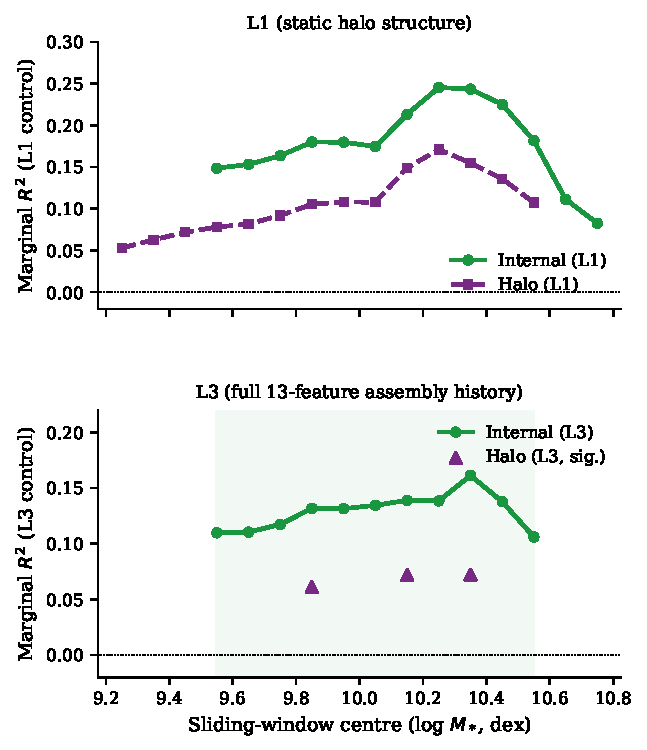
\includegraphics[width=\textwidth]{outputs/figures/fig02_phase_diagram.pdf}
\caption{Intermediate-mass growth phase diagram.
  Internal (solid) and halo L1 marginal $R^2$ (upper) and L3 marginal $R^2$
  (lower) versus sliding-window centre (0.5-dex windows, step 0.1 dex).
  L1 significant interval: 9.55--10.65 dex (13 windows).
  L3 significant interval (green shading): 9.55--10.55 dex (\WindowNWindowsL{}
  consecutive significant windows), where internal $\Rmarg$ is individually
  significant.
  L3 halo collapses to 3 non-contiguous windows (triangles); the halo L3
  markers are shown as disconnected triangles, with no connecting line, because
  the significant halo intervals are non-contiguous.
  Vertical dotted lines mark the L3 significant interval (9.55--10.55 dex).
\label{fig:phase_diagram}}
\end{figure*}

\subsection{Internal Leads Halo Across the Entire Regime}
\label{sec:flat_gap}

Figure~\ref{fig:gap} shows the shared-bootstrap paired gap
$\delta = R^2(\mathrm{L3+internal}) - R^2(\mathrm{L3+halo})$ at each
sliding window centre.
The assembly-history baseline cancels algebraically in this test, giving a
direct internal-vs-halo comparison under full gravitational control; this
algebraic cancellation makes the paired gap the paper's most statistically
robust diagnostic, immune to uncertainty in the absolute level of the
baseline.

\begin{deluxetable}{lcccc}
\tablecaption{L3 paired gap (internal $-$ halo) by window
  centre.\label{tab:gap}}
\tablehead{
  \colhead{Centre (dex)} & \colhead{$n$} &
  \colhead{$\delta$} & \colhead{95\% CI} & \colhead{Sig}
}
\startdata
9.25--9.45 & \nodata & $<0$ & spans zero & ns \\
\textbf{9.55} & 2,393 & $+0.071$ & $[+0.049, +0.095]$ & * \\
9.65 & 2,213 & $+0.067$ & $[+0.042, +0.085]$ & * \\
9.75 & 2,023 & $+0.066$ & $[+0.042, +0.089]$ & * \\
9.85 & 1,908 & $+0.071$ & $[+0.047, +0.094]$ & * \\
9.95 & 1,747 & $+0.072$ & $[+0.047, +0.091]$ & * \\
10.05 & 1,566 & $+0.071$ & $[+0.043, +0.093]$ & * \\
10.15 & 1,459 & $+0.067$ & $[+0.046, +0.084]$ & * \\
10.25 & 1,407 & $+0.065$ & $[+0.049, +0.087]$ & * \\
10.35 & 1,337 & $+0.089$ & $[+0.051, +0.101]$ & * \\
10.45 & 1,228 & $+0.071$ & $[+0.044, +0.094]$ & * \\
10.55 & 1,158 & $+0.052$ & $[+0.030, +0.085]$ & * \\
10.65 & 1,026 & $+0.026$ & $[+0.016, +0.071]$ & * \\
\textbf{10.75} & 836  & $+0.016$ & $[+0.004, +0.061]$ & * \\
$\geq10.85$ & \nodata & ns & \nodata & \\
\enddata
\tablecomments{$*$ denotes 95\% CI entirely above zero.}
\end{deluxetable}

\begin{figure}[t!]
\centering
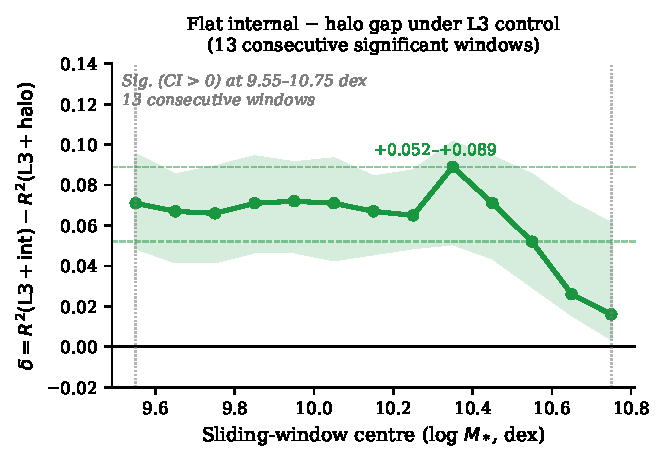
\includegraphics[width=\columnwidth]{outputs/figures/fig03_paired_gap.pdf}
\caption{Flat internal--halo paired gap across the regime.
  L3 shared-bootstrap paired gap $\delta = R^2(\mathrm{L3+internal}) -
  R^2(\mathrm{L3+halo})$ versus window centre with 95\% CI shading.
  The paired gap is significant over 9.55--10.75 dex (\PairedGapNWindows{}
  consecutive windows), extending two windows beyond the 9.55--10.55 dex
  internal interval, because the geometry cancellation in the paired test
  removes baseline noise.
  Gap ranges $\PairedGapLo$--$\PairedGapHi$ with no strong mass dependence.
\label{fig:gap}}
\end{figure}

The gap is significant at every window from 9.55 to 10.75 dex ---
\PairedGapNWindows{} consecutive windows.
The geometry cancellation extends this significant range two windows beyond
the 9.55--10.55 dex internal interval: internal $\Rmarg$ becomes ns at 10.65
dex, but the paired
gap persists to 10.75 dex because the baseline cancels algebraically in the
shared-bootstrap paired test.
As for the marginal interval, the 9.55-dex lower bound of this gap interval
reflects catalog recoverability rather than a physical threshold; only the
upper bound marks a physical transition.
Across that upper edge the population changes character: between the
9.55--10.55 dex interval and the 10.55--10.75 dex band the median specific
star-formation rate drops from $\log\mathrm{sSFR} = -9.63$ to $-10.96$, the
quenched fraction rises from $0.035$ to $0.498$, and the median black-hole mass
increases by $1.51$ dex --- the 10.55-dex boundary coincides with the onset of
black-hole--associated quenching, which is why it, unlike the lower edge, is a
physical transition.

The gap is also remarkably \textit{flat}: across 1.2 dex of stellar mass,
$\delta$ ranges $\PairedGapLo$ to $\PairedGapHi$ with no strong peaking or
edge effect.
Internal's advantage over halo is a stable property of the entire
intermediate-mass regime, not an artefact of a single peak mass.
The simulation jackknife confirms this: the ordering internal $>$ halo
under L3 is preserved at all 9.55--10.55 dex windows in 27/27
leave-one-out configurations.

\subsection{Mechanistic Decomposition}
\label{sec:mechanism}

\subsubsection{Gas mass is the dominant surviving internal carrier}

To identify which features within the internal family carry the residual
signal, we apply permutation importance to L3-residualized columns at the
mid-mass regime, with each feature regressed against the 13 assembly-history
variables and replaced by its OLS residual before shuffling
(Table~\ref{tab:importance}).

\begin{deluxetable}{lcccc}
\tablecaption{L3-residualized permutation importance, mid-mass growth
  ($n = \MidMassN$).\label{tab:importance}}
\tablehead{
  \colhead{Feature} & \colhead{Raw imp.} &
  \colhead{L3-resid imp.} & \colhead{95\% CI} & \colhead{Retention}
}
\startdata
\multicolumn{5}{c}{\textit{Internal class}} \\
\hline
$\log M_\mathrm{gas}$ & $0.145$ & $\mathbf{+0.027}$ & $[+0.017, +0.038]$ & 19\% \\
All other internal & $\leq0.002$ & $\approx0$ & spans zero & absorbed \\
\hline
\multicolumn{5}{c}{\textit{Halo class}} \\
\hline
$\fstar = M_*/M_\mathrm{sub}$ & $0.037$ & $\mathbf{+0.031}$ & $[+0.021, +0.044]$ & 84\% \\
$\log\lambda$ (spin) & $0.017$ & $+0.007$ & $[+0.002, +0.013]$ & 41\% \\
$\log V_\sigma$ (veldisp) & \nodata & $+0.005$ & $[+0.001, +0.011]$ & \nodata \\
$\log M_\mathrm{sub}$ & $0.031$ & $\approx0$ & spans zero & absorbed \\
\enddata
\end{deluxetable}

The result is unambiguous: gas mass is the sole internal feature retaining
significant importance after full gravity residualization.
All other internal features --- SFR, sSFR, stellar mass, metallicity,
half-mass radius --- are absorbed by the L3 assembly-history.
Stellar-to-halo fraction $\fstar$ is the most gravity-resistant feature in
the entire analysis, retaining 84\% of its raw permutation importance after
L3 residualization.

\begin{figure}[t!]
\centering
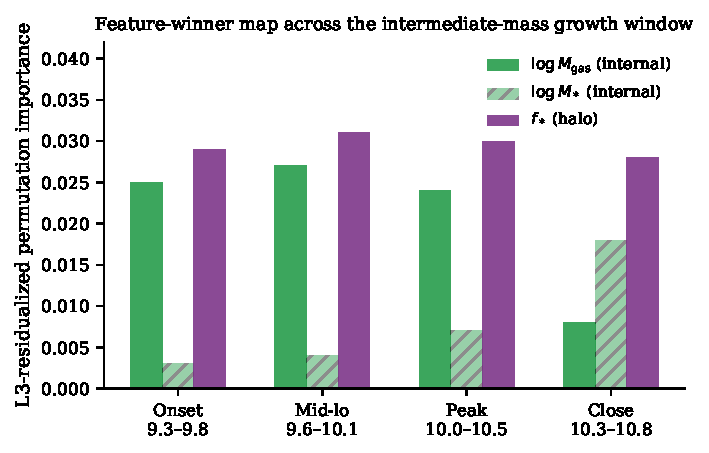
\includegraphics[width=\columnwidth]{outputs/figures/fig04_feature_winner.pdf}
\caption{Feature-winner map across the intermediate-mass growth regime.
  L3-residualized permutation importance at four window positions.
  Gas mass (dark green) dominates the internal class at onset through peak;
  stellar mass (hatched) is the sole surviving internal feature at the close.
  $\fstar$ (purple) is the stable halo carrier throughout.
\label{fig:features}}
\end{figure}

\subsubsection{Assembly timing, not mergers, is the main absorbing
gravitational channel}

\begin{deluxetable*}{lccccccc}
\tablecaption{Assembly ablation map, mid-mass growth
  ($n = \MidMassN$).\label{tab:ablation}}
\tablehead{
  \colhead{Ablated family} & \colhead{Features removed} &
  \colhead{Geom baseline} &
  \colhead{Int marg} & \colhead{Recovery} &
  \colhead{Halo marg} & \colhead{Halo rec.}
}
\startdata
None (full L3) & \nodata & $0.185$ & $0.135^*\,[0.095, 0.184]$ & \nodata & $\LThreeHaloMarg^*$ & \nodata \\
\textbf{Mergers} & $n_\mathrm{merg}$, $n_\mathrm{maj}$, $t_\mathrm{last\,maj}$ & $0.183$ & $0.135^*\,[0.097, 0.183]$ & $\mathbf{\AblationMergerRecovery}$ & $0.081^*$ & $-0.002$ \\
\textbf{Long accretion} & $\Delta\log M_{sl12}$, $\Delta\log M_{sl16}$ & $0.170$ & $0.149^*\,[0.108, 0.193]$ & $\mathbf{\AblationLongAccretionRecovery}$ & $0.095^*$ & $+0.012$ \\
\textbf{Peak/halfmass} & peak mass ratio, $t_{1/2}$ & $0.160$ & $0.161^*\,[0.122, 0.208]$ & $\mathbf{\AblationTimingRecovery}$ & $0.107^*$ & $+0.024$ \\
\enddata
\tablecomments{Recovery $= \Delta R^2_{\mathrm{marg,int}} =$ ablated marginal $-$
  full L3 marginal.}
\end{deluxetable*}

\begin{figure}[t!]
\centering
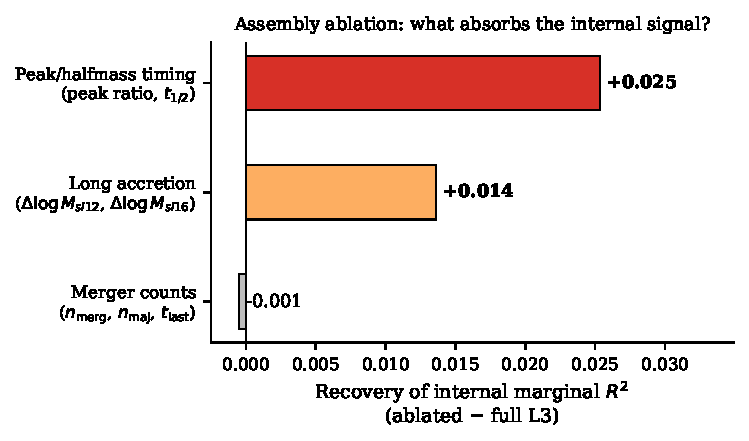
\includegraphics[width=\columnwidth]{outputs/figures/fig05_ablation.pdf}
\caption{Assembly ablation map.
  Internal class marginal $R^2$ recovery when each gravity-feature family
  is removed from the L3 assembly-history: merger features (recovery
  $+0.000$), late accretion ($+0.014$), peak/halfmass timing ($+0.026$).
  Assembly timing is the strongest gravitational absorber of the internal
  signal; merger counts carry zero.
\label{fig:ablation}}
\end{figure}

From the weak-L1 control (static halo position only) to the full 13-feature L3
baseline, the internal-family marginal for mid-mass growth falls from $0.308$ to
$0.135$, so $0.173$ in $R^2$ is absorbed by assembly history.
Peak mass ratio and half-mass assembly snapshot together account for
\AblationTimingPct\% of the absorbed internal marginal.
Late-lookback accretion (4--8 Gyr) accounts for a further
\AblationLongAccretionPct\%.
Merger counts recover zero internal signal: the residual internal signal in
the mid-mass regime is entirely merger-count-independent.
Together, the three tested components account for approximately 29\% of the
absorbed internal signal at mid-mass (timing: \AblationTimingPct\%, long
accretion: \AblationLongAccretionPct\%, mergers: 0\%); the remaining
$\approx 71\%$ is not resolved to specific assembly-history features in this
decomposition.
Extending the ablation to the early-accretion band (1--2 Gyr lookback,
$\Delta\log M_\mathrm{halo}$ over 4 and 8 SubLink steps) does not localize the
remainder: the recent-accretion pair recovers $+0.009$ ($\approx 7\%$ of the
full-L3 internal marginal) and each feature alone $\leq 7\%$, with no single
assembly feature exceeding the half-mass epoch's $\approx 16\%$. Because the 13
assembly features are strongly collinear, these recoveries overlap rather than
add, so the absorbed signal does not concentrate in any one feature. We therefore
interpret the unresolved $\approx 71\%$ as distributed, correlated
assembly-history structure spread across the manifold --- a decomposition limit
of the present 13-feature L3 control, not a single missing absorber and not a
claim of fundamental irreducibility.

The gravitational clock most correlated with baryonic growth information is
\textit{when} the halo assembled most of its mass and whether it has been
gaining or losing mass since its peak, not how many mergers occurred.

\subsubsection{The internal channel is not mediated by stellar efficiency}

We add $\fstar$ directly to the L3 assembly-history baseline and re-run the
assembly-history control.
Adding $\fstar$ raises the baseline from $R^2 = 0.185$ to $0.251$ ---
stellar efficiency carries $+0.066\ R^2$ beyond the 13 assembly features.

\begin{deluxetable}{lcccc}
\tablecaption{Effect of adding $\fstar$ to L3 baseline, mid-mass
  growth.\label{tab:fstar}}
\tablehead{
  \colhead{Class} & \colhead{L3 marg} &
  \colhead{L3+$\fstar$ marg} & \colhead{95\% CI} & \colhead{Verdict}
}
\startdata
internal & $\LThreeInternalMarg^*$ & $\mathbf{\FstarInternalMarg^*}$ & $[\FstarInternalCILo, \FstarInternalCIHi]$ & \textbf{SURVIVES} \\
halo     & $\LThreeHaloMarg^*$ & $\FstarHaloMarg$ & $[-0.030, +0.064]$ & \textbf{ABSORBED} \\
env      & $0.024$ (ns) & $0.013$ (ns) & $[-0.032, +0.060]$ & ns \\
\enddata
\end{deluxetable}

Internal's marginal drops from \LThreeInternalMarg{} to \FstarInternalMarg{} but remains
significant, with a CI entirely above zero.
Halo's marginal drops to \FstarHaloMarg{} and becomes non-significant:
halo's surviving L3 signal is entirely mediated through stellar-to-halo
fraction.
Under L3+$\fstar$, internal leads halo 5-to-1 ($\FstarInternalMarg$ vs.\
$\FstarHaloMarg$), compared to 1.6-to-1 under L3 alone --- adding one
baryonic efficiency feature exposes a qualitative difference in what the
two classes are tracking.

\subsection{The Nature of the Residual Internal Signal}
\label{sec:gasnature}

What kind of information does the surviving gas signal carry? Four targeted
tests on the TNG SubLink sample, using the same five-fold ridge cross-validation
and shared bootstrap, characterize it (Figure~\ref{fig:mechanism}).

\begin{figure*}[t!]
\centering
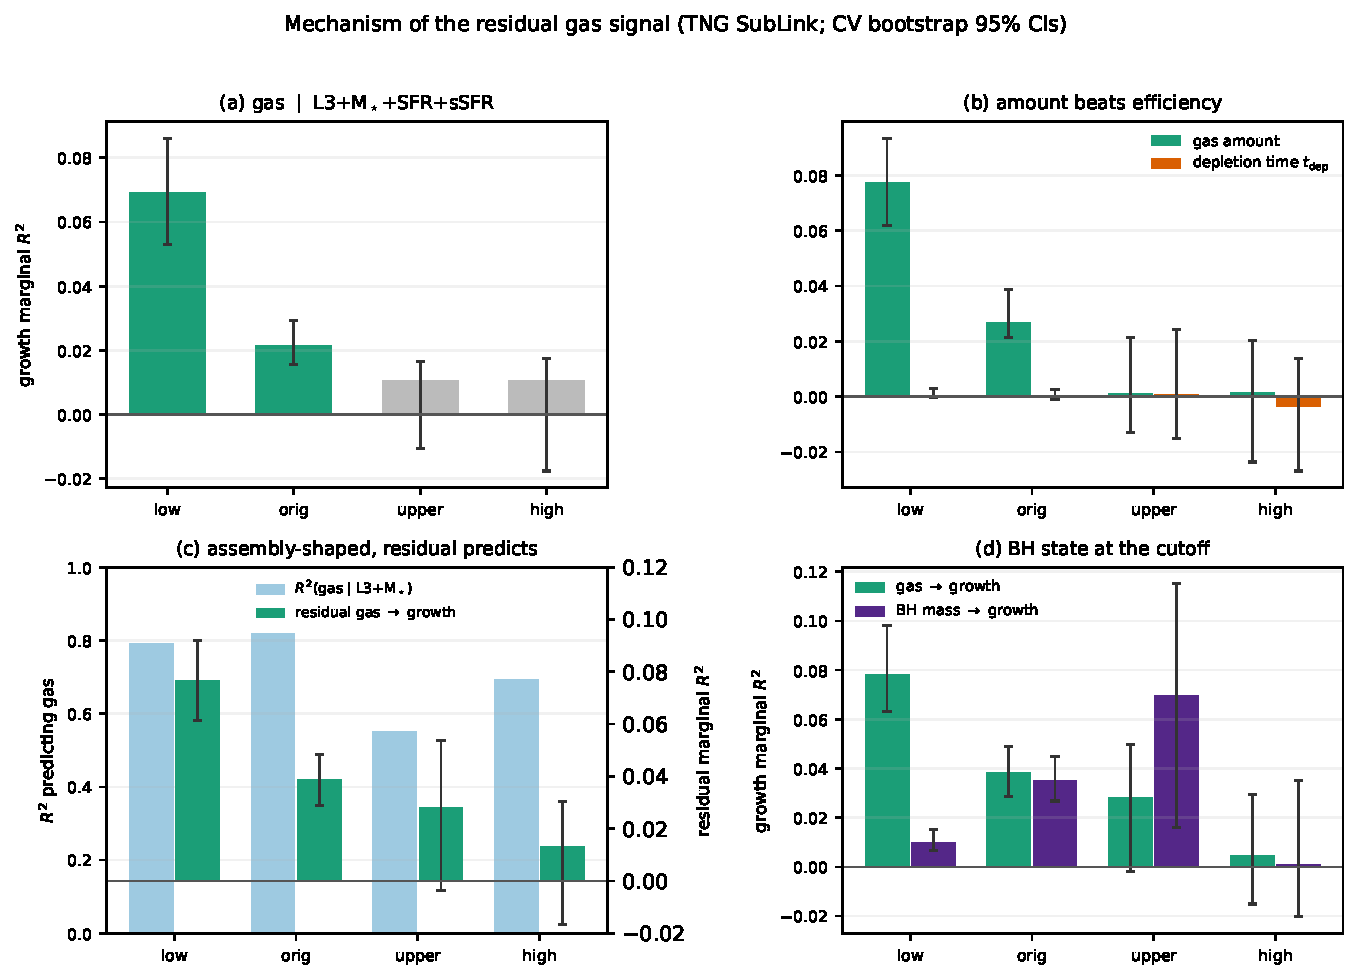
\includegraphics[width=\textwidth]{outputs/referee/fig_mechanism_compact.pdf}
\caption{Mechanism of the residual gas signal in TNG (SubLink trees), by
  stellar-mass regime: low ($9.0$--$9.55$), \textit{orig} ($9.55$--$10.55$), upper
  transition ($10.55$--$10.75$), and high ($>10.75$ dex). Error bars are shared
  paired-bootstrap 95\% confidence intervals throughout.
  \textbf{(a)}~The gas-mass marginal for future stellar growth survives joint
  control for the early star-formation rate, specific star-formation rate,
  \emph{and} stellar mass on top of the L3 assembly-history baseline --- significant
  at low and intermediate mass (green), not individually significant above the
  cutoff (grey).
  \textbf{(b)}~The carrier is gas \emph{amount}, not efficiency: gas mass adds
  growth information beyond the depletion time
  $t_\mathrm{dep}=M_\mathrm{gas}/\mathrm{SFR}$, whereas $t_\mathrm{dep}$ adds
  essentially nothing once gas amount is included.
  \textbf{(c)}~The reservoir is strongly shaped by assembly history --- the
  L3$+M_\star$ baseline predicts $\log M_\mathrm{gas}$ at $R^2\simeq0.8$ (light
  bars, left axis) --- yet the orthogonal residual gas still predicts growth
  (green, right axis): assembly-shaped, but not exhausted.
  \textbf{(d)}~Near the upper boundary the informative predictor changes hands from
  gas to black-hole mass --- used as a black-hole/quenching \emph{state} proxy, not
  a direct feedback-energy measurement: the gas$\rightarrow$growth marginal fades
  while the BH-mass$\rightarrow$growth marginal peaks at the upper transition.
\label{fig:mechanism}}
\end{figure*}

First, the signal is not merely the present star-forming state. Adding the
early-epoch star-formation rate, specific star-formation rate, and stellar mass
to the L3 control, the gas-mass marginal for stellar growth remains positive:
$+0.022\,[+0.015, +0.029]$ over 9.55--10.55 dex and $+0.069\,[+0.053, +0.086]$
at lower mass. Once gas is included the current star-formation rate adds
essentially nothing, so the carrier is the gas reservoir rather than the
instantaneous conversion rate.

Second, the signal is gas \emph{amount}, not gas-use efficiency. Replacing gas
amount with the depletion time $t_\mathrm{dep} = M_\mathrm{gas}/\mathrm{SFR}$
(which is independent of stellar mass), gas amount adds beyond $t_\mathrm{dep}$
($+0.077$ at low mass, $+0.027$ over the interval) while $t_\mathrm{dep}$ adds
nothing once gas amount is controlled. The predictive content is the amount of
available fuel, not how efficiently it is currently being consumed.

Third, the reservoir is strongly shaped by halo assembly history but not
exhausted by it. The L3 baseline plus stellar mass predicts
$\log M_\mathrm{gas}$ at $R^2 \simeq 0.8$ over this mass range --- dominated by
halo mass and assembly timing --- yet the gas component orthogonal to that
prediction still predicts future growth (residual-gas marginal $+0.077$ at low
mass, $+0.039$ over the interval). Assembly history substantially determines the
gas reservoir, but a predictive baryonic residual remains.

Fourth, near the upper boundary the informative predictor changes. Using
catalog-level black-hole proxies --- black-hole mass and accretion rate, taken
as state indicators rather than direct feedback-energy measurements ---
black-hole/quenching state carries the growth signal at the upper transition
(10.55--10.75 dex; BH-mass marginal $+0.070\,[+0.016, +0.115]$), where the gas
marginal is not individually significant, and it carries the quenching signal at
intermediate mass (BH-mass AUC marginal $+0.032\,[+0.025, +0.040]$), where gas
does not. The high-mass bins are underpowered and the population there is largely
quenched by $z = 0$ ($\gtrsim 95\%$ above 10.75 dex); this is a change in which
proxy is informative, not a disappearance of the gas channel.

\subsection{Robustness}
\label{sec:robustness}

The ordering internal $>$ halo $>$ env for mid-mass growth is preserved
in 27/27 LOO jackknife configurations; the same holds for mid-mass
quenching and for all three targets in the whole-sample analysis, so no
single simulation drives any verdict.
Replacing $\log M_\mathrm{sub}$ with $\log V_\mathrm{max}$ in the L1
control raises the baseline ($R^2 = 0.175$ vs.\ $0.004$) but preserves
the ordering: internal $+0.137^*\,[+0.092, +0.179]$ vs.\ halo
$+0.075^*\,[+0.034, +0.116]$, a ratio of $\approx 1.8\times$ compared to
$1.3\times$ under $M_\mathrm{sub}$.
The lead is robust to the choice of halo structural variable.

The residual internal signal is also not an artifact of the linear ridge model.
Repeating the mid-mass ($\WindowLoL \le \logM/M_\odot \le \WindowHiL$)
L3-controlled stellar-growth comparison with non-linear regressors, the
internal-family marginal remains positive with a random forest
($+0.120\,[+0.102, +0.132]$) and histogram gradient boosting
($+0.119\,[+0.100, +0.135]$), compared with $+0.139\,[+0.119, +0.153]$ for ridge,
and gas mass remains the leading internal feature in all three by
permutation importance. We adopt ridge for the main analysis for transparency
and paired-bootstrap stability, not because the result depends on linearity.


\subsection{Cross-Simulation Comparison at a Matched (L1) Control}
\label{sec:cross_family}

The mechanistic results of Sections~\ref{sec:window}--\ref{sec:mechanism}
are based on TNG SubLink.
To test family robustness, we run the L1 sliding-window mass scan on SIMBA
spatial (Figure~\ref{fig:cross_family}), restricting to the growth and
quenching targets.

At a matched L1 control, the two simulations differ sharply in the growth
channel: SIMBA's L1 growth-channel internal-family marginal does not reach
robust significance (scan peak $+0.080$, 95\% CI spanning zero), and any SIMBA
growth signal is weak and fragmented, whereas TNG's is a clean $+0.245$ over
the same control. The SIMBA L1 internal--halo paired gap for growth is
correspondingly significant at only two isolated mass centres.

The quenching channel is the opposite. At the same L1 control SIMBA's
internal-family quenching marginal is large and broadly significant (peak
marginal AUC $+0.141^*$ at 10.15 dex, significant from 9.65 to 10.75 dex;
Table~\ref{tab:simba_quench}; halo also significant, peak $+0.127^*$), whereas
TNG's quenching marginal is small ($+0.060^*$ at L1). The same-control L1
contrast in the quenching channel is thus $\sim$2.4$\times$ in SIMBA's favour.

\begin{deluxetable}{lcccccc}
\tablecaption{SIMBA L1 quenching marginal AUC, selected
  windows.\label{tab:simba_quench}}
\tablehead{
  \colhead{Centre (dex)} & \colhead{$n$} &
  \colhead{Int marg AUC} & \colhead{Sig} &
  \colhead{Halo marg AUC} & \colhead{Sig}
}
\startdata
9.65 & 1,225 & $+0.068$ & * & $+0.045$ & ns \\
9.85 & 1,098 & $+0.111$ & * & $+0.111$ & * \\
\textbf{10.15} & 855 & $\mathbf{+\SimbaQuenchPeak}$ & * & $+0.127$ & * \\
10.25 & 825 & $+0.125$ & * & $+0.096$ & * \\
10.35--10.45 & \nodata & $+0.123$--$+0.117$ & * & $+0.100$--$+0.083$ & * \\
10.75 & 550 & $+0.086$ & * & $+0.083$ & * \\
$\geq10.85$ & \nodata & ns & & ns & \\
\enddata
\end{deluxetable}

The TNG quenching marginal is weak at every control level: peak L1 AUC
$+0.060^*$ at 9.85 dex, tightening further under L3, confirming that TNG's
beyond-gravity signal does not lie in the quenching channel
(Figure~\ref{fig:cross_family}, lower-left).
We compare the two simulations only at the shared L1 control; we deliberately
do \emph{not} set SIMBA's L1 quenching marginal against TNG's more conservative
L3 marginal, as that would confound the target-channel question with the depth
of the gravitational control.

At a matched L1 control, then, the two feedback models express their residual
beyond-gravity internal information through different target channels: in TNG
it concentrates in stellar growth (the upper-bounded intermediate-mass regime
of Section~\ref{sec:window}), whereas in SIMBA it concentrates in quenching
(broadly significant L1 band, peak marginal AUC $+0.141$), with SIMBA's growth
signal weak and fragmented.

We stress the scope of this contrast.
The TNG branch supports the full mechanistic decomposition --- static
position versus accretion history versus full assembly history --- via
merger-tree matching.
The SIMBA branch supports only a same-control L1 target-channel contrast:
SubLink-equivalent merger trees are unavailable for SIMBA at CAMELS resolution,
so we make \emph{no} claim of an L3-controlled residual in SIMBA.
The SIMBA result should be read as evidence that the target channel of the
beyond-gravity signal differs across feedback models at a matched static
control, not as a matched mechanistic replication of the TNG assembly-history
decomposition.

\begin{figure*}[t!]
\centering
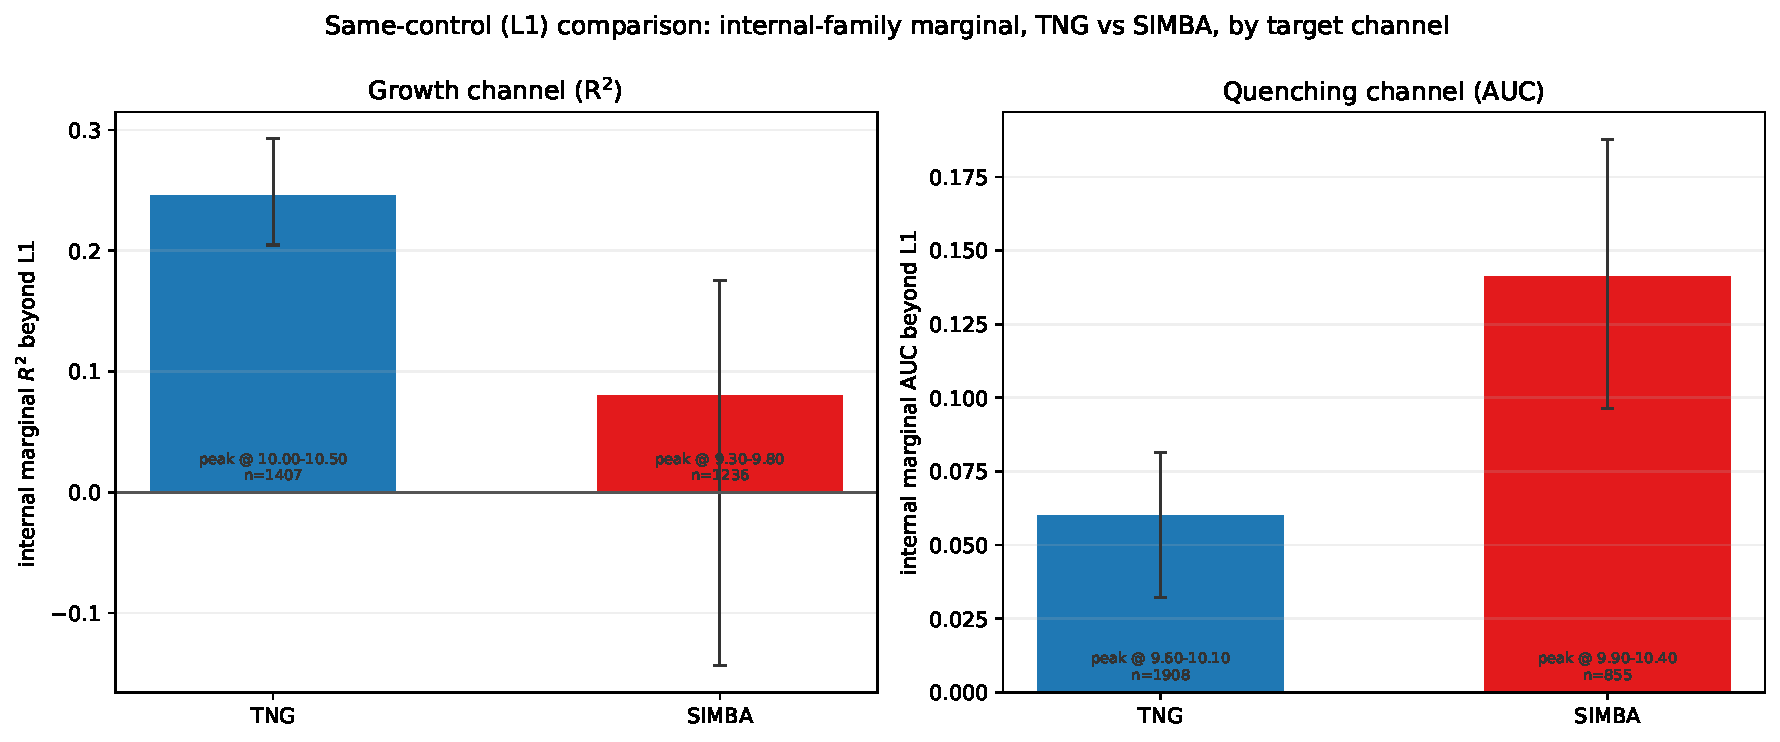
\includegraphics[width=\textwidth]{outputs/referee/fig_simba_same_control.pdf}
\caption{Cross-simulation comparison at a matched L1 (static-halo) control:
  internal-family marginal for TNG (blue) and SIMBA (red), by target channel.
  \textit{Left}: future stellar growth (marginal $R^2$ beyond L1). TNG carries a
  clean internal signal ($+0.245\,[+0.205, +0.293]$), whereas SIMBA's is weak and
  not robustly significant (peak $+0.080$, 95\% CI spanning zero).
  \textit{Right}: quenching (marginal AUC beyond L1). The ordering reverses ---
  SIMBA's internal quenching marginal is large
  ($+\SimbaQuenchPeak^*\,[+0.096, +0.188]$) while TNG's is small
  ($+0.060^*\,[+0.032, +0.081]$), an L1-vs-L1 amplitude ratio of
  $\sim$2.4$\times$ in SIMBA's favour. Error bars are shared paired-bootstrap
  95\% confidence intervals; the peak mass band and sample size are annotated on
  each bar. Tree-based assembly (L3) controls are unavailable for SIMBA at CAMELS
  resolution, so the comparison is made only at the shared L1 control and no SIMBA
  L3 residual is claimed.
\label{fig:cross_family}}
\end{figure*}

% ---------------------------------------------------------------------------
\section{\textbf{Discussion}}
\label{sec:discussion}

\subsection{Interpretation: From Fuel-Limited to Quenching-Limited Growth}

Across an upper-bounded intermediate-mass regime (significant under L3 up to
$\logM/M_\odot \simeq 10.55$ in this suite), a galaxy's baryonic state at
$z \approx 0.77$ carries \textit{predictive} information about its $z = 0$
stellar growth that is not fully captured by its gravitational trajectory ---
even given static position, accretion rate over multiple lookback windows,
peak mass, half-mass assembly epoch, merger counts, and major-merger timing.
The overall picture is a transition from a \textit{fuel-limited} regime at
low-to-intermediate mass, where the residual gas reservoir predicts future
growth, to a \textit{quenching-limited} regime near and above the upper
boundary, where black-hole/quenching state becomes the informative channel.

We do not interpret the lower edge as a physical onset: below $\sim 9.55$ dex
the recovery of the gas signal is limited by catalog-floor and resolution
effects (\S\ref{sec:window}), so the apparent low-mass onset is a recovery edge
rather than a physical transition. Whether a genuine low-mass change exists
(e.g.\ a greater role for environment via ram pressure, tidal stripping, or
filamentary gas supply \citep{dekel2009}) cannot be settled at this resolution.

The upper boundary near $\sim 10.55$ dex is physically meaningful: there the
predictive structure shifts to black-hole/quenching state (traced by
catalog-level black-hole proxies, \S\ref{sec:gasnature}) and the population is
largely quenched by $z = 0$, so the regime is bounded above by the onset of
quenching rather than by assembly history alone.
In the intermediate regime below it, the current gas \emph{amount} carries
predictive information that the 13 tested gravitational descriptors do not
fully recover.
The upper boundary is defined within the CAMELS CV setup and may shift modestly
with volume and resolution (see \S\ref{sec:caveats}).

The regime has a carrier structure within it
(Section~\ref{sec:mechanism}): gas mass dominates the surviving internal
signal from the onset through the peak, but shifts to accumulated stellar
mass near the close.
This is consistent with observational evidence that cold-gas content is a
strong predictor of near-future star formation at intermediate mass
\citep{saintonge2017,davies2019}, and with a picture where, toward higher
mass, the gas-to-growth link is increasingly absorbed by gravitational
history while the galaxy's position in the quenching trajectory ---
reflected in accumulated stellar mass \citep{genel2019} --- retains an
independent predictive contribution.

\textbf{Observational prediction.}
This residual gas-reservoir signal is not merely a simulation result --- it is
a quantitative prediction testable on real galaxy surveys.
The prediction is: in observed galaxies at $9.55 \lesssim \logM \lesssim 10.55$
(roughly $z \lesssim 0.1$), cold-gas mass should retain marginal predictive
power for stellar growth $\sim 1$--$2$ Gyr later, above and beyond what
halo-mass proxies (weak-lensing mass, group membership, velocity dispersion)
already predict.
The xGASS and xCOLD\,GASS surveys \citep{saintonge2017} observe total cold-gas
content (HI + H$_2$) for star-forming galaxies in precisely this stellar-mass
range, with group-membership and halo-mass proxies available from companion
catalogs.
A marginal-predictive battery run on xGASS/xCOLD\,GASS --- with halo-mass
proxies as the assembly-history control and cold-gas mass as the test predictor
--- would constitute a direct observational test of the regime.
If the signal survives in observed galaxies, it would establish that the
predictive contribution of gas content relative to halo assembly is not an
artifact of the CAMELS feedback prescriptions.

\subsection{What the Result Does Not Mean}

Three misreadings of the result should be avoided.
It is not anti-gravitational: the assembly-history baseline accounts for
roughly half the internal family's signal in this regime (L3 retention
$\approx 43\%$ from an L1 baseline near 100\%), so halo assembly history
remains the dominant information source and the internal signal is a residual
beyond it.
It does not mean that only baryonic information matters here: halo structure
also survives L3 in the regime, albeit in fewer mass bins and with a smaller
marginal.
Nor is it universal: the residual is confined to the intermediate regime ---
recovery-limited at low mass and underpowered at high mass --- and the
whole-sample tie of Section~\ref{sec:whole_sample} is real.

\subsection{Why Assembly Timing is the Main Gravitational Competitor}

The assembly ablation result (Section~\ref{sec:mechanism}) constrains which
part of the halo assembly-history baseline most overlaps with the internal
predictive signal.
Peak mass ratio and half-mass assembly snapshot account for
\AblationTimingPct\% of the absorbed internal advantage; late-lookback
accretion accounts for a further \AblationLongAccretionPct\%; merger counts
account for 0\%.
Together these three decomposed components account for $\sim 29\%$ of the
absorbed signal at mid-mass --- a meaningful but minority fraction, indicating
that the dominant absorbing channels within L3 are not yet individually
identified.

Peak mass ratio and half-mass assembly epoch together encode the galaxy's
gravitational \textit{maturity} in the sense of \citet{lacey1993} ---
when it assembled most of its mass and whether it has been on a declining
trajectory since \citep{wechsler2006,mao2018}.
A galaxy that peaked early and has been stripped carries different
predictive content from one still near its peak mass, even at the same
present-day halo mass.

This timing information partially \textit{overlaps} with the baryonic signal
because a galaxy near its mass peak is more likely to have a well-stocked
gas reservoir at the relevant epoch \citep{saintonge2017}.
The overlap is partial and predictive, not a causal decomposition --- which
is precisely why the internal signal survives after ablating those features.

Merger counts do not participate in this overlap.
The number of mergers experienced, or when the last major merger occurred,
does not substantially predict the current gas mass or the future growth
rate, net of the other assembly descriptors.
The residual internal signal in the mid-mass regime is
merger-count-independent.

\subsection{The $\fstar$ Boundary}

Adding $\fstar$ to the assembly-history baseline absorbs halo's surviving
L3 marginal entirely while leaving internal's intact.
This is a sharp result: internal carries baryonic growth information that is
orthogonal to both the halo assembly-history baseline and the integrated
efficiency of star formation.
Halo's surviving gravity-controlled signal, by contrast, was tracking
formation efficiency all along.

The physical implication is that the baryonic channel cannot be reduced to
``the galaxy happens to be efficient at forming stars.''
Whatever the gas-mass signal captures --- current fueling conditions,
feedback state, gas phase --- it is not recoverable from the
stellar-to-halo ratio record even in combination with 13 assembly features.

\subsection{Why the Family Contrast Is Meaningful, and What It Does Not Yet Prove}

The SIMBA result is not a robustness check for the TNG growth result; it is
a different measurement.
SIMBA shows that a beyond-gravity baryonic signal exists in SIMBA too, but
it is concentrated in quenching rather than stellar growth.
At this matched L1 control, the simplest reading is a feedback-model difference
in target-channel expression (scoped to L1, not a mechanistic claim): TNG's
prescription leaves more independent information in the fuel-to-growth channel,
while SIMBA's stronger wind quenching leaves more in the quenching channel.

In TNG, the mechanistic decomposition is clean: we have merger-tree
assembly-history control escalating from static position through full
assembly history, assembly ablations, and the $\fstar$ augmentation test.
In SIMBA, we have a target-channel comparison at L1 only.
The SIMBA result is best understood as evidence for a family-level
difference in which baryonic outcome carries the beyond-gravity signal, not
as a parallel mechanistic decomposition.
Resolving whether the SIMBA quenching signal survives an equivalent L3
assembly-history control requires SIMBA SubLink-equivalent trees, which are
not currently available at CAMELS resolution.

\subsection{Caveats}
\label{sec:caveats}

Several limitations apply to these results.
Even at its best, the internal predictor family explains only
$R^2 \approx 0.31$ of mid-mass growth variance, leaving $\approx 69\%$
unexplained.
This residual likely reflects stochastic processes not recoverable from
snapshot features, finite resolution suppressing small-scale ISM physics,
the compression of internal state into six scalar features, and genuine
physical stochasticity.

The CAMELS CV suite uses $25\, h^{-1}\,\mathrm{Mpc}$ boxes with $256^3$
particles. At the low-mass end the lower edge of the regime is a
floor-encoding / resolution-limited recovery boundary (\S\ref{sec:window}), not
a physical onset: a small tail of unresolved objects whose gas feature sits at
the catalog floor destabilizes the low-mass fit. We do not have a
higher-resolution CAMELS run with which to test convergence, so we report the
9.55-dex onset as a recovery edge and the upper boundary near 10.55 dex as the
physically meaningful edge.
The small box also coarsely samples large-scale modes, so the environmental
null --- environment carries no marginal beyond L1 in any window --- is
specific to this CV volume and the environment features used here, and we do
not claim it as a general result.
The CV suite holds astrophysical parameters fixed, so results are valid for the
specific TNG and SIMBA prescriptions at CAMELS resolution; the effect of varying
feedback strength is not explored.
Finally, direct AGN feedback-energy fields are not present in the CAMELS group
catalogs used here, so the high-mass transition is characterized through
black-hole state proxies (black-hole mass and accretion rate), not a
feedback-energy measurement.
Relatedly, the loaded group-catalog products provide total subhalo gas mass but
no phase-separated cold or star-forming gas reservoir (no cold-, neutral-, or
molecular-gas mass field is present), so our gas predictor is total gas. The
observational prediction is correspondingly framed in terms of total
gas-reservoir content and should be tested with cold-gas surveys; isolating the
cold or star-forming phase on the simulation side would require particle-level or
value-added data beyond the loaded catalogs.

On the SIMBA side, SubLink-equivalent merger trees are not available, so L3
assembly-history control cannot be applied. The SIMBA quenching result
(Section~\ref{sec:cross_family}) is at L1 only.
All findings are correlational throughout: predictive advantage means a
family carries information about the target, not that it causes the outcome.
The 13 L3 assembly-history features were selected for physical breadth ---
covering static position, multiple accretion-rate lookbacks, peak-mass epoch,
half-mass assembly, and merger history --- rather than optimized for
predictive importance against the internal target.
A feature-selected or higher-dimensional assembly-history control could absorb
a larger share of the internal signal, though the robustness of the surviving
signal in the permutation-importance test (gas mass) and the $\fstar$ boundary
check suggests this result is not dominated by L3 feature-set
sensitivity.
Finally, SubLink matching excludes galaxies that merge or are disrupted
between $z = 0.77$ and $z = 0$, leaving the mid-mass sample modestly biased
toward galaxies with surviving central descendants.
Excluded galaxies --- those undergoing mergers or disruption --- likely have
disturbed gas reservoirs and atypically elevated star-formation rates relative
to the retained sample; including them would tend to suppress rather than
amplify the internal marginal signal near the 9.55 dex recovery onset.
The lower edge of the regime is therefore, if anything, a conservative
estimate.

% ---------------------------------------------------------------------------
\section{\textbf{Conclusions}}
\label{sec:conclusions}

We have compared three predictor families --- internal galaxy properties,
halo structural properties, and environmental measures --- as predictors of
stellar growth, quenching, and halo growth in CAMELS CV IllustrisTNG
($n = \TNGSubLinkN$) and SIMBA ($n = \SIMBASpatialN$) central galaxies,
with escalating controls for halo structural position and assembly history.
The main findings are:

\begin{enumerate}
  \item \textbf{No feature family leads consistently}: every cell in the
    $3 \times 3$ score matrix is a statistical tie in both TNG and SIMBA.
    The overall tie pattern is simulation-robust but does not describe the
    full mass-regime structure.

  \item \textbf{An upper-bounded intermediate-mass gas-reservoir regime}:
    under the full 13-feature assembly-history control, internal galaxy state
    retains significant marginal predictive power for stellar growth up to
    $\logM/M_\odot \simeq 10.55$ (\WindowNWindowsL{} consecutive significant
    windows over the catalog-recovered interval $9.55$--$10.55$ dex, peak
    internal marginal $R^2 = \WindowPeakMarg^*$, 43\% retention at the fixed
    mid-mass window). The lower edge is a floor-encoding/resolution-limited
    recovery boundary, not a physical onset; outside this regime feature-family
    advantages are largely assembly-history-mediated.

  \item \textbf{Internal leads halo across $9.55$--$10.75$ dex}: the
    shared-bootstrap paired gap (internal $-$ halo) under L3 is positive and
    significant at every window in this range (\PairedGapNWindows{} consecutive
    windows, $\PairedGapLo$--$\PairedGapHi$, all CIs positive), extending two
    windows beyond the $9.55$--$10.55$ dex internal interval.
    The gap is flat --- it does not peak at a single mass.

  \item \textbf{Gas mass is the dominant surviving internal carrier}: the
    only internal feature retaining significant permutation importance after
    L3 residualization.
    Its assembly-history-residualized importance is 19\% of its raw
    importance, broadly consistent with the family-level retention.

  \item \textbf{Assembly timing, not mergers, is the main absorbing gravity
    channel}: removing peak mass ratio and half-mass assembly snap from L3
    recovers \AblationTimingPct\% of the absorbed internal marginal;
    removing merger counts recovers 0\%.
    The mid-mass internal signal is merger-count-independent.

  \item \textbf{The internal channel is not mediated by stellar efficiency}:
    adding $\fstar$ to the L3 assembly-history absorbs halo's surviving
    marginal entirely ($\LThreeHaloMarg^* \to \FstarHaloMarg$ ns) but leaves
    internal's intact ($\LThreeInternalMarg^* \to \FstarInternalMarg^*\,
    [\FstarInternalCILo, \FstarInternalCIHi]$).
    Internal carries baryonic growth information orthogonal to both
    gravitational assembly history and galaxy formation efficiency.

  \item \textbf{A beyond-gravity baryonic signal appears in both simulation
    families, but its target-channel expression differs}: in TNG it is
    expressed through stellar growth (\WindowNWindowsL{}-window L3 interval;
    paired gap over \PairedGapNWindows{} windows,
    $\PairedGapLo$--$\PairedGapHi$); in SIMBA, at a matched L1 control, the
    stronger signal appears in quenching (10+ window L1 band, peak marginal AUC
    $= \SimbaQuenchPeak^*$), while the SIMBA growth signal is fragmented and
    not robustly significant.
    The TNG branch supports the full mechanistic decomposition; the SIMBA
    branch supports a target-channel contrast.
    Whether the SIMBA quenching signal survives full assembly-history
    control requires merger-tree equivalents not yet available for SIMBA at
    CAMELS resolution.
\end{enumerate}

A detailed accounting of what is and is not claimed by these results ---
including explicit statements on the absence of causal claims, universal
mass thresholds, observational inference, and cross-simulation replication
--- is given in Appendix~\ref{app:earned}.
Directions for follow-up (SIMBA merger-tree control, volume and resolution
tests, and redshift evolution of the regime) are collected in
Appendix~\ref{app:future}.

% ---------------------------------------------------------------------------
\begin{acknowledgments}
The author thanks the open-source scientific Python community for the
libraries underlying this work: NumPy, SciPy, pandas, scikit-learn,
matplotlib, and tqdm.
The CAMELS simulations were produced by the CAMELS collaboration and are
publicly available through the Flatiron Institute data portal.
CAMELS IllustrisTNG uses the IllustrisTNG galaxy-formation model developed
by the IllustrisTNG collaboration; CAMELS SIMBA uses the SIMBA model
developed by R.\ Dav\'{e} and collaborators.
\end{acknowledgments}

% ---------------------------------------------------------------------------
\section*{Data and Code Availability}

The CAMELS simulation data used in this work are publicly available at
\url{https://camels.readthedocs.io}.
All analysis code, figure-generation scripts, and the compiled paper are
available at \url{https://github.com/kunalb541/Camels}.

% ---------------------------------------------------------------------------
\appendix
\raggedbottom  % appendix pages sit naturally (white space to the bottom) rather than stretching between items

% ---------------------------------------------------------------------------
\section{\textbf{Additional Mechanism and Robustness Diagnostics}}
\label{app:diagnostics}

The compact mechanism summary in the main text (Figure~\ref{fig:mechanism}) and the
cross-simulation comparison (Figure~\ref{fig:cross_family}) are distilled from a
broader set of diagnostics, reproduced here in full so that the supporting evidence
is visible rather than asserted. Unless noted, all reuse the paper pipeline
(five-fold ridge cross-validated $R^2$ for growth, logistic cross-validated AUC for
quenching, shared paired-bootstrap 95\% confidence intervals) on the TNG SubLink
sample.

The gas reservoir is separated from the present star-forming state in
Figure~\ref{fig:app_gasvssfr}: controlling jointly for the early star-formation
rate, specific star-formation rate, and stellar mass on top of L3, the gas-mass
marginal for future growth remains $+0.022\,[+0.015, +0.029]$ over 9.55--10.55 dex
and $+0.069\,[+0.053, +0.086]$ at lower mass. The raw gas-\emph{fraction} marginal
is inflated by its stellar-mass denominator ($+0.121$); the leakage-free gas-mass
quantity is the $+0.022$ value quoted throughout.

\begin{figure*}[htbp]
\centering
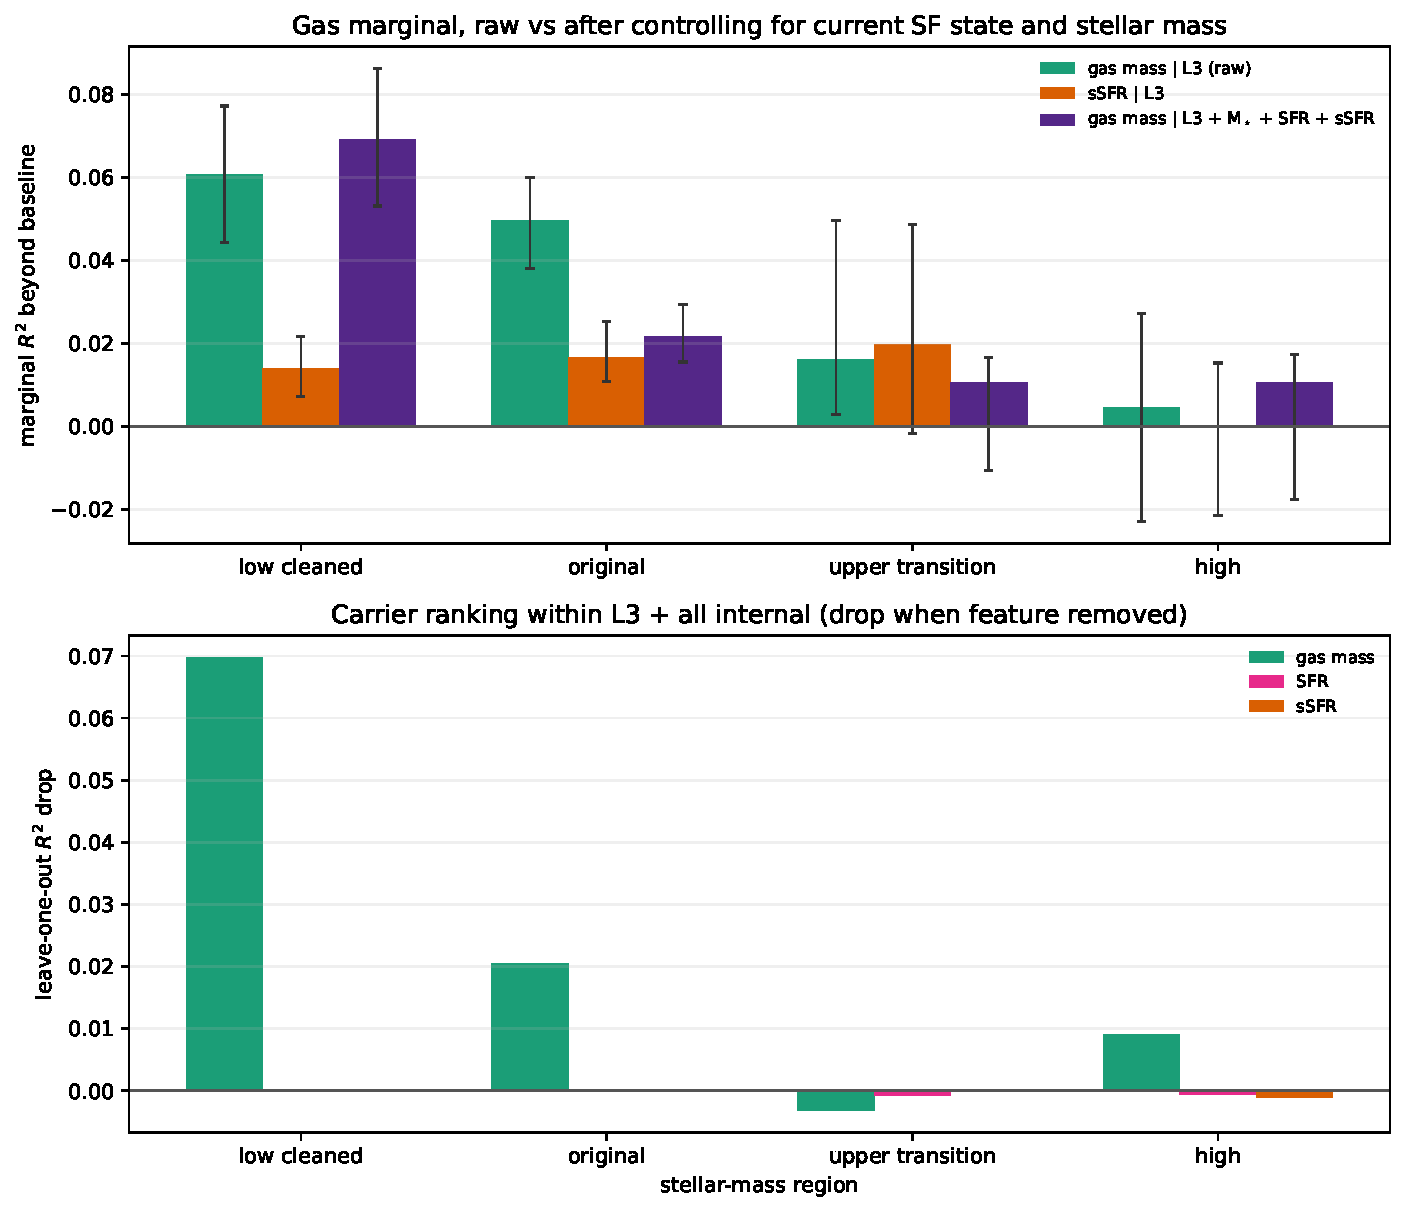
\includegraphics[width=\textwidth]{outputs/referee/fig_gas_vs_sfr_discriminator.pdf}
\caption{Gas-reservoir versus current-star-formation discriminator. After
  controlling for the early SFR, sSFR, and stellar mass, the gas-mass marginal for
  future growth stays positive ($+0.022$ over the interval, $+0.069$ at low mass);
  the raw gas-fraction marginal ($+0.121$) is inflated by its stellar-mass
  denominator and is shown only to disclose that inflation.
\label{fig:app_gasvssfr}}
\end{figure*}

Figure~\ref{fig:app_depletion} contrasts gas amount with the depletion time
$t_\mathrm{dep}=M_\mathrm{gas}/\mathrm{SFR}$ (constructed to be independent of
stellar mass). Gas amount adds beyond $t_\mathrm{dep}$ ($+0.077$ at low mass,
$+0.027$ over the interval), whereas $t_\mathrm{dep}$ adds essentially nothing once
gas amount is included ($\simeq\!-0.000$): the predictive content is the amount of
available fuel, not the instantaneous conversion efficiency.

\begin{figure*}[htbp]
\centering
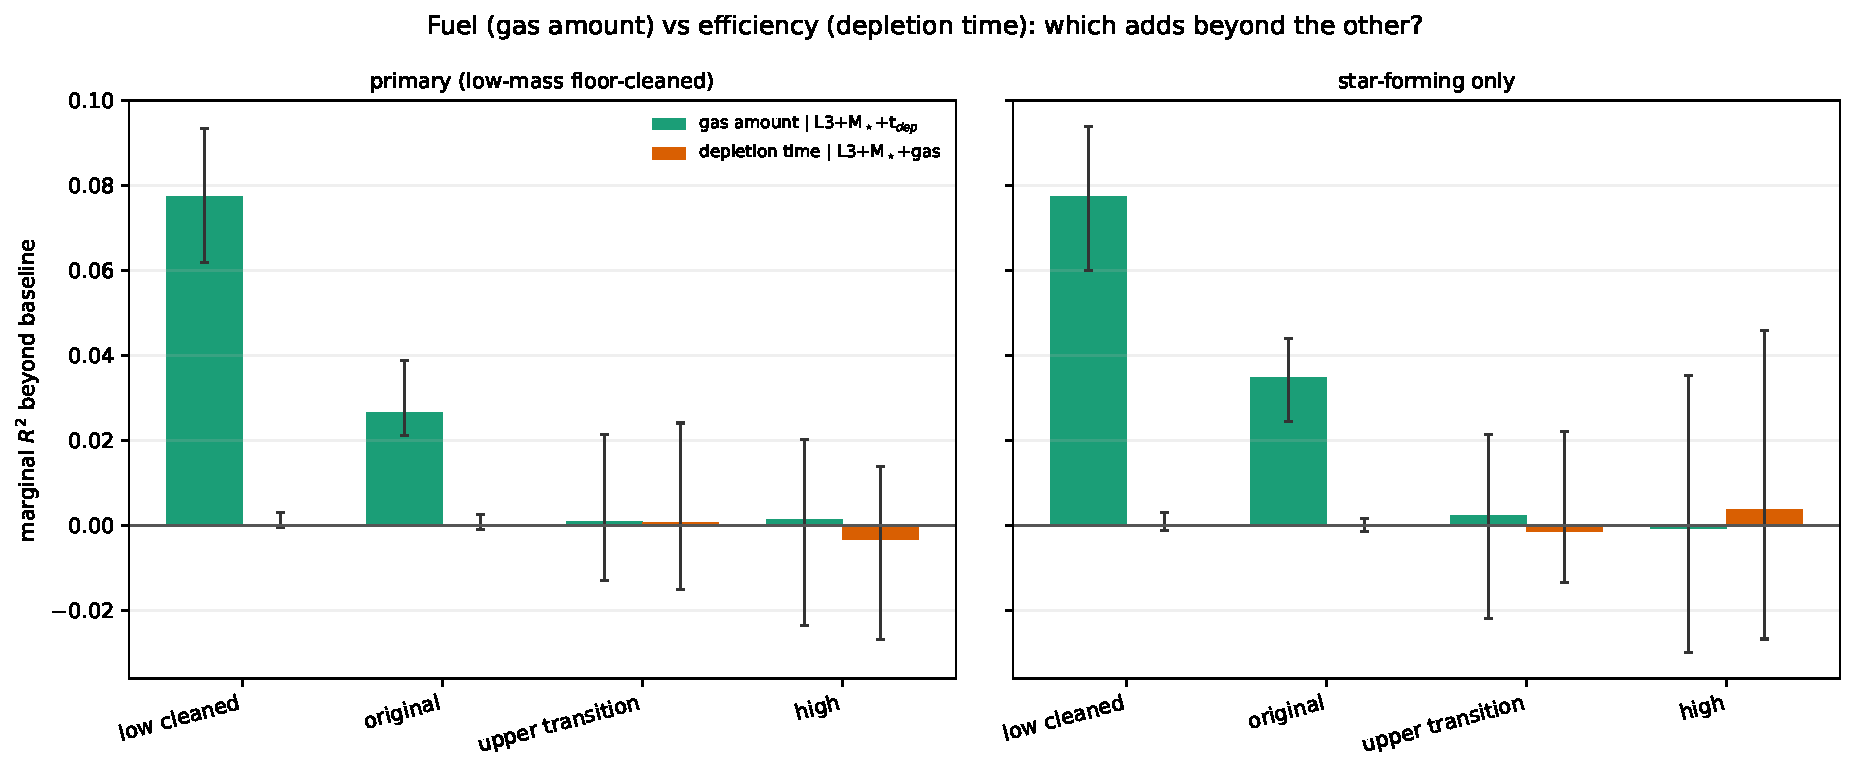
\includegraphics[width=\textwidth]{outputs/referee/fig_depletion_time.pdf}
\caption{Gas amount versus depletion time. Gas amount carries growth information
  beyond $t_\mathrm{dep}=M_\mathrm{gas}/\mathrm{SFR}$, while $t_\mathrm{dep}$ adds
  essentially nothing once gas amount is controlled --- the signal is fuel amount,
  not conversion efficiency.
\label{fig:app_depletion}}
\end{figure*}

The reservoir's encoding by assembly history is quantified in
Figure~\ref{fig:app_gaspred}: the L3$+M_\star$ baseline predicts
$\log M_\mathrm{gas}$ at $R^2 = 0.793$ (low) and $0.818$ (interval) --- it is largely
set by halo mass and assembly timing --- yet the gas component orthogonal to that
prediction still predicts future growth ($+0.077$ low, $+0.039$ interval). The
reservoir is assembly-shaped but not exhausted.

\begin{figure*}[htbp]
\centering
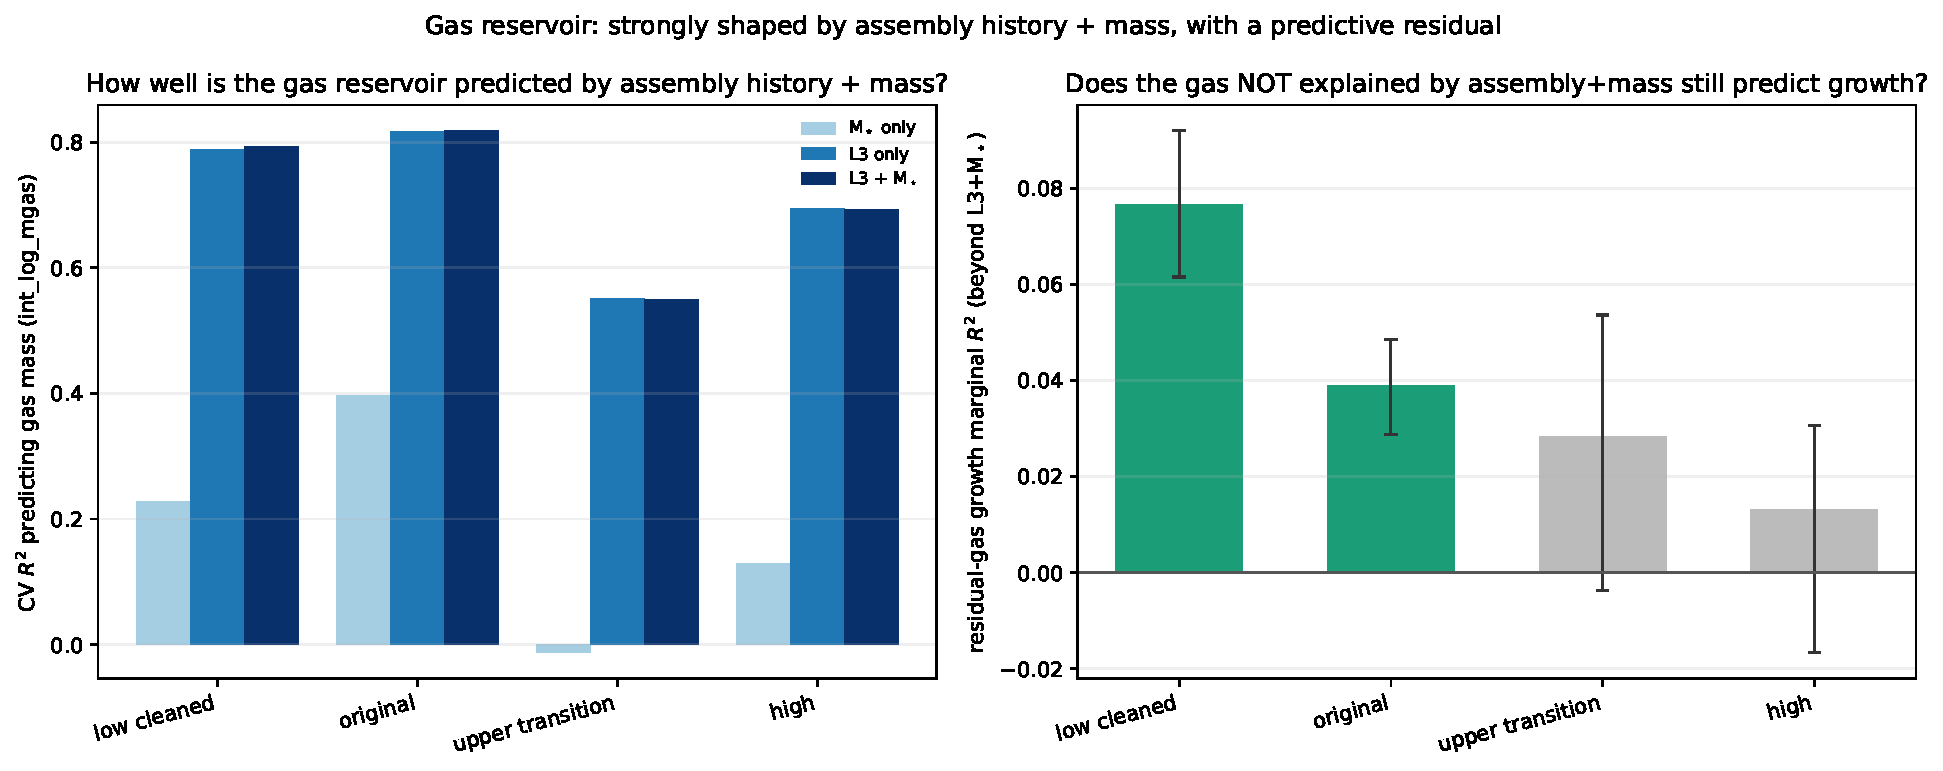
\includegraphics[width=\textwidth]{outputs/referee/fig_gas_predictability_by_assembly.pdf}
\caption{Assembly encoding of the gas reservoir. The L3$+M_\star$ baseline predicts
  the reservoir at $R^2\simeq0.8$, but the orthogonal residual gas retains a positive
  growth marginal ($+0.077$ low, $+0.039$ interval): the reservoir is shaped by halo
  assembly history without being fully determined by it.
\label{fig:app_gaspred}}
\end{figure*}

Figure~\ref{fig:app_bh} follows the black-hole proxies (mass and accretion rate,
used as state indicators rather than feedback-energy measurements). The BH-mass
growth marginal peaks at the upper transition ($+0.070\,[+0.016, +0.115]$, where the
gas marginal is not individually significant), and the BH-mass quenching marginal is
significant at intermediate mass ($\mathrm{AUC}\ +0.032\,[+0.025, +0.040]$); above
10.75 dex the population is $\gtrsim 95\%$ quenched by $z = 0$.

\begin{figure*}[htbp]
\centering
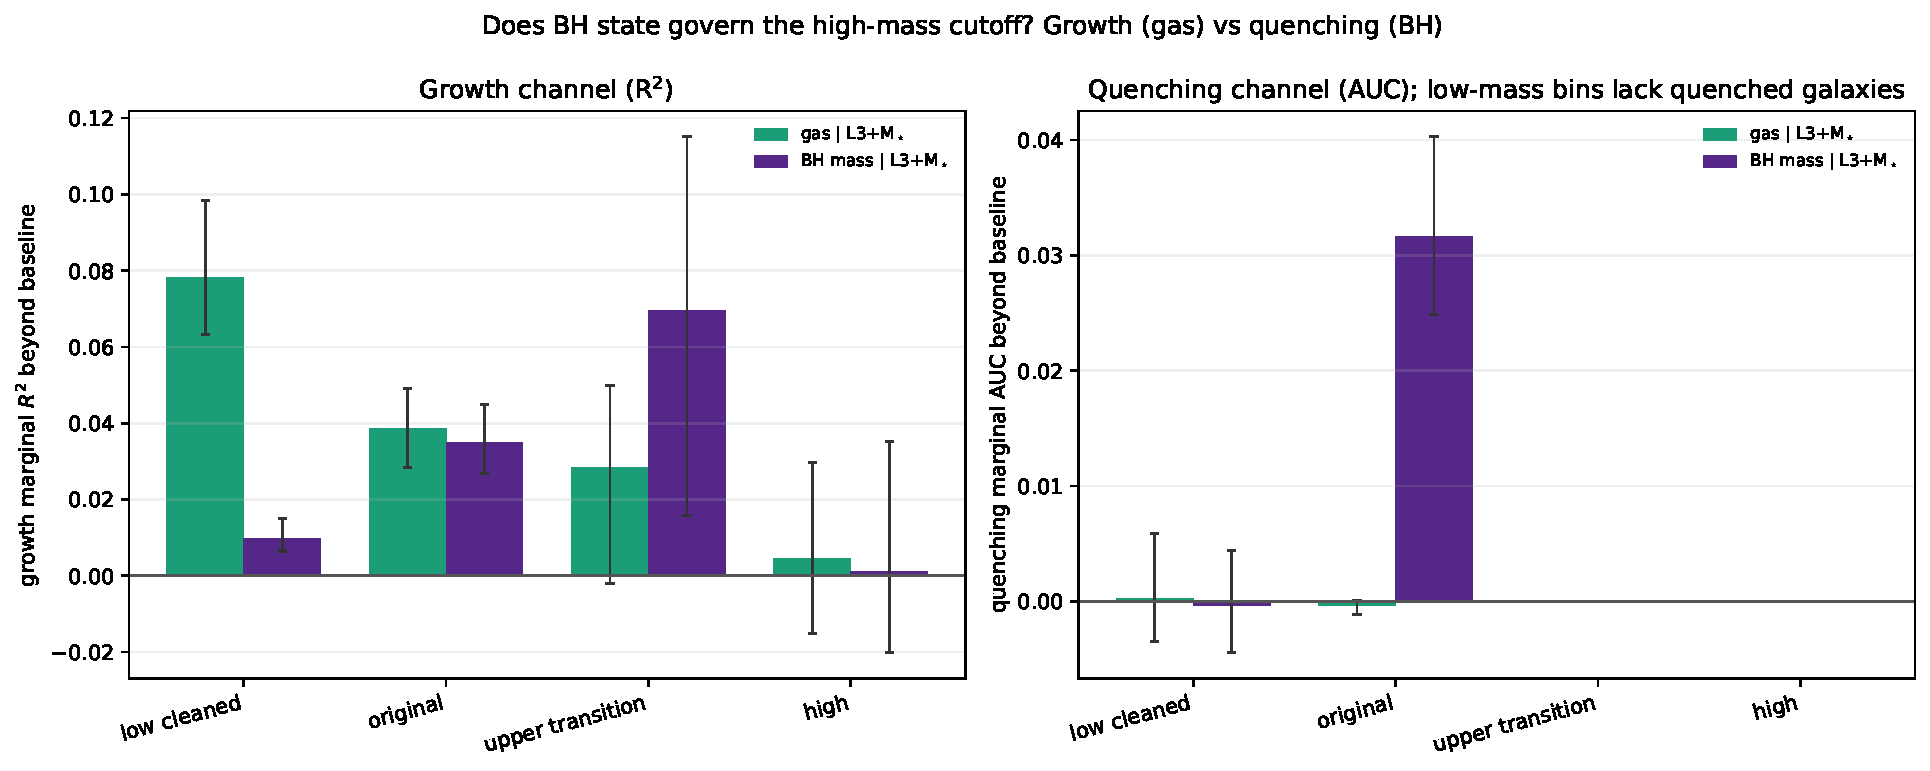
\includegraphics[width=\textwidth]{outputs/referee/fig_bh_absorber.pdf}
\caption{Black-hole state at the upper transition. Black-hole mass (a state proxy,
  not a feedback-energy measurement) carries the growth signal at the upper
  transition and the quenching signal at intermediate mass --- precisely where the
  gas marginal is not individually significant.
\label{fig:app_bh}}
\end{figure*}

A coarsened-exact-matching test of the gas$\rightarrow$growth effect at fixed stellar
mass, halo mass and assembly history is shown in Figure~\ref{fig:app_matched}. A
positive effect is recovered where matching is feasible --- low mass,
$\mathrm{ATT}=+0.138\,[+0.105, +0.172]$ dex at borderline covariate balance
($|\mathrm{SMD}|=0.14$) --- while the intermediate and upper regimes are
matching-infeasible (insufficient high-gas/low-gas overlap at fixed covariates). We
treat this as supportive robustness at low mass rather than a global causal estimate,
which is why it appears here rather than in the main text.

\begin{figure*}[htbp]
\centering
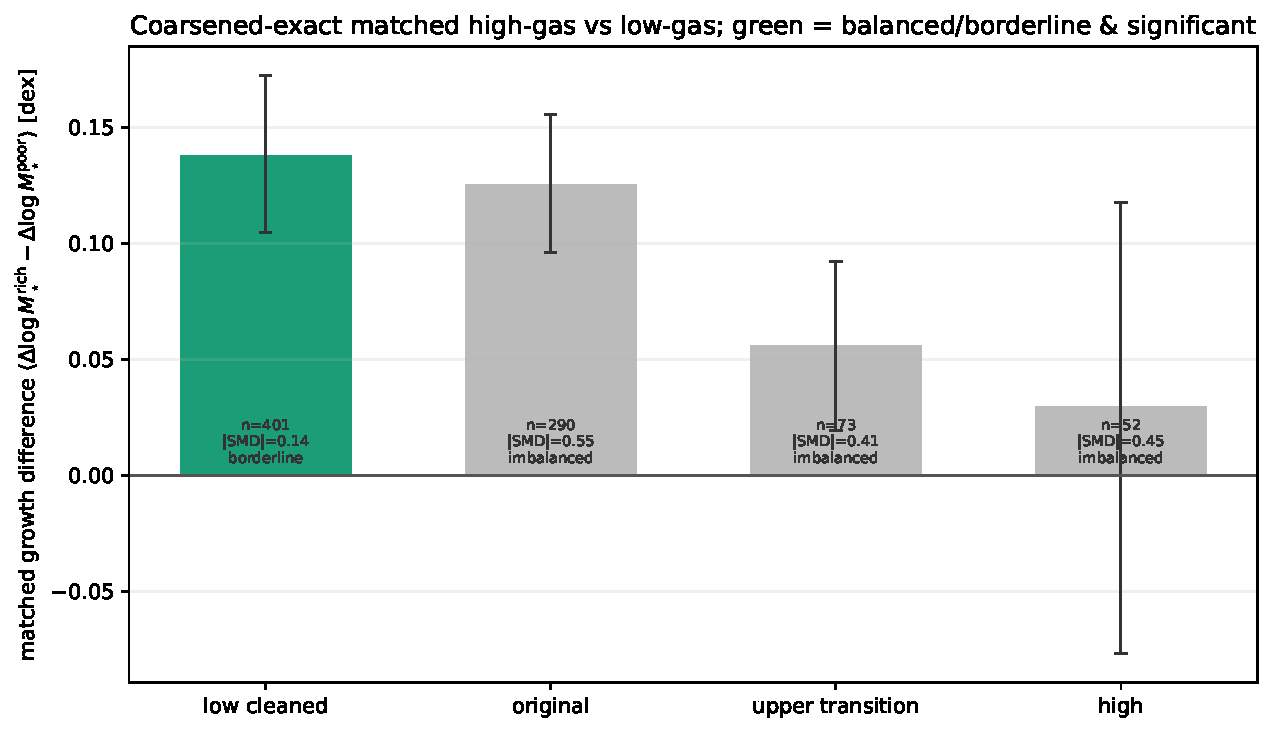
\includegraphics[width=\textwidth]{outputs/referee/fig_matched_gas_pairs.pdf}
\caption{Coarsened-exact-matched gas$\rightarrow$growth test. At low mass, where
  high-gas and low-gas galaxies can be matched on stellar mass, halo mass and
  assembly history, the matched effect is $\mathrm{ATT}=+0.138$ dex (borderline
  balance, $|\mathrm{SMD}|=0.14$); the higher-mass regimes lack sufficient overlap to
  match. Supportive robustness, not a global causal estimate.
\label{fig:app_matched}}
\end{figure*}

Finally, Figure~\ref{fig:app_winsor} establishes that the lower edge is not a
physical threshold. Below 9.55 dex the full-sample gas marginal is destabilised by a
few objects whose gas feature is pinned at the catalog floor (estimate $+0.005$ with
a meaningless interval $[-0.279, +0.010]$); deleting that tail gives $+0.061$, and,
crucially, \emph{winsorizing} the floor-encoded feature without removing any object
recovers $+0.057$ --- matching the onset band ($+0.061$). The lower edge is therefore
a floor-encoding / resolution-limited measurement edge.

\begin{figure}[htbp]
\centering
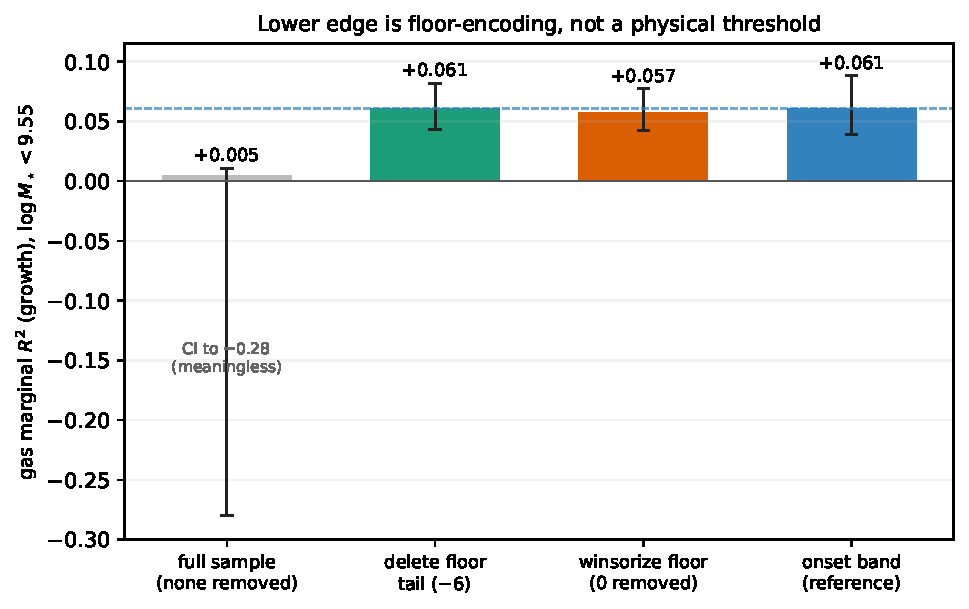
\includegraphics[width=\columnwidth]{outputs/referee/fig_lower_edge_winsorization.pdf}
\caption{Lower-edge floor encoding. Deleting ($-6$ objects) or winsorizing
  ($32$ objects, none removed) the floor-pinned gas feature recovers the same gas
  marginal ($+0.061$ / $+0.057$) as the onset reference band ($+0.061$), whereas the
  raw full-sample estimate ($+0.005$) carries a meaningless interval reaching
  $-0.28$. The lower edge is a floor-encoding / resolution-limited measurement edge,
  not a physical threshold.
\label{fig:app_winsor}}
\end{figure}

% ---------------------------------------------------------------------------
\section{\textbf{Scope of Claims}}
\label{app:earned}

\noindent\textbf{Earned in this paper.}
\begin{itemize}[leftmargin=*,itemsep=2pt]
  \item \textit{No single feature family is globally best across the tested
    targets.}  Across the whole-sample target matrix, environment, internal,
    and halo families are all competitive; the ranking changes with both
    target and mass regime.

  \item \textit{An upper-bounded mid-mass growth regime exists in TNG in which
    internal galaxy state adds predictive information beyond the tested
    gravitational prescription.}  In the TNG SubLink branch, internal features
    retain positive marginal $R^2$ for future stellar growth after conditioning
    on the full 13-feature assembly-history control.

  \item \textit{That internal advantage is regime-specific, not global.}
    The beyond-gravity signal is concentrated in a bounded intermediate-mass
    interval rather than extending across the full sample.

  \item \textit{The internal-minus-halo gap is positive across that interval
    under the full TNG gravity control.}  Internal state is not merely
    surviving control; it remains ahead of halo structure across the interval.

  \item \textit{Gas mass is the dominant surviving internal carrier.}
    Within the internal family, gas mass is the main load-bearing predictor
    after the full gravity control.

  \item \textit{Halo assembly timing is the main absorbing gravitational
    channel.}  Peak-mass ratio and half-mass assembly timing recover
    substantially more absorbed internal signal than merger-count variables.

  \item \textit{Merger counts do not explain the internal growth signal.}
    Removing merger-count features in the ablation recovers essentially none
    of the absorbed internal marginal.

  \item \textit{The surviving internal signal is not mediated by stellar-to-halo
    fraction $\fstar$.}  Adding $\fstar$ to the baseline absorbs halo's residual
    but leaves the internal signal positive and significant.

  \item \textit{The matching-method confound is real and quantitatively
    important.}  Spatial matching inflates the geometry baseline by
    $\SpatialInflation\times$ relative to merger-tree matching; mechanistic
    interpretation should rest on the SubLink/TNG branch.

  \item \textit{SIMBA supports a cross-family channel contrast, but not a
    matched mechanistic replication.}  TNG expresses the beyond-gravity signal
    primarily in growth; SIMBA expresses it primarily in quenching.
\end{itemize}

\medskip\noindent\textbf{Not earned in this paper.}
\begin{itemize}[leftmargin=*,itemsep=2pt]
  \item \textit{A universal internal-state superiority claim.}
    The paper shows a bounded, regime-specific TNG result, not a general
    dominance of internal state across galaxy evolution targets.

  \item \textit{Universal mass boundaries.}
    The quoted interval edges are earned within the CAMELS setup and should not
    be read as universal physical thresholds independent of volume, resolution,
    or feedback model; the lower edge in particular is resolution-limited.

  \item \textit{A causal claim.}
    These are predictive and decomposition results.  The paper shows information
    beyond the tested gravitational prescription, not causal independence from
    gravity.

  \item \textit{A statement that gravity is unimportant.}
    The full assembly-history baseline explains a large share of the signal;
    the surviving internal component is a residual beyond that baseline, not a
    replacement for it.

  \item \textit{A clean mechanistic replication in SIMBA.}
    Without tree-based control for SIMBA, the SIMBA result is comparative
    support, not a matched mechanistic replication.

  \item \textit{A resolution- or volume-independent result.}
    The paper does not establish that the interval location or width is
    unchanged under larger boxes or higher resolution.

  \item \textit{A direct observational claim.}
    This is a simulation result on feature families and predictive structure,
    not an observational inference about real galaxies.

  \item \textit{Proof that gas physics is independent of halo history.}
    The paper shows residual predictive information after the tested gravity
    controls, not absolute independence between gas content and assembly.
\end{itemize}

% ---------------------------------------------------------------------------
\section{\textbf{Future Directions}}
\label{app:future}

The two most direct extensions are:

\textbf{SIMBA merger-tree control.}  The SIMBA branch uses only spatial
matching, which inflates halo baselines by $\SpatialInflation\times$ and
prevents a direct L3-equivalent test.
Constructing SubLink-like trees for SIMBA-CAMELS would enable a fully
symmetric comparison and determine whether the SIMBA quenching signal
survives a 13-feature assembly-history control.

\textbf{Volume and resolution.}  Results come from $25\,h^{-1}$\,Mpc boxes
with $256^3$ particles.  Running the same analysis on larger CAMELS
extensions will determine whether the predictive interval shifts or broadens
at higher mass.

Two further simulation directions are worth pursuing: (\textit{i})~repeating
the sliding-window scan at $z \approx 0.5$ and $1.0$ to track whether the
regime evolves as assembly history accumulates; (\textit{ii})~tracking net
gas inflows and outflows along individual TNG trajectories to identify
whether the gas-mass signal reflects accretion or feedback-driven depletion.
The direct observational test of the upper-bounded gas-reservoir regime via xGASS/xCOLD\,GASS
\citep{saintonge2017} is discussed and formulated as a prediction in
Section~\ref{sec:discussion}.

% ---------------------------------------------------------------------------
\section{\textbf{Supporting Tables}}
\label{app:tables}

\begin{table}[H]
\centering
\caption{Predictive scores by stellar mass regime, TNG SubLink.
  Bold = WINNER at raw (uncontrolled) level; the assembly-history-controlled
  gap for mid-mass growth is $\PairedGapLo$--$\PairedGapHi$ across
  \PairedGapNWindows{} consecutive windows (Table~\ref{tab:gap}).
  \label{tab:mass_splits}}
\resizebox{\columnwidth}{!}{%
\begin{tabular}{llccccc}
\toprule
Target & Mass bin & $n$ & env & halo & internal & Verdict \\
\midrule
\multirow{3}{*}{Growth $R^2$}
  & Low ($<9.5$)    & \LowMassN  & 0.166 & 0.160 & 0.040 & TIE \\
  & Mid (9.5--10.5) & \MidMassN  & 0.083 & \MidMassHaloR & \textbf{\MidMassInternalR} & \textbf{WINNER: internal} \\
  & High ($\geq10.5$) & \HighMassN & 0.068 & 0.107 & 0.118 & TIE \\
\midrule
\multirow{3}{*}{Quenching AUC}
  & Low ($<9.5$)    & \LowMassN  & 0.645 & 0.704 & 0.681 & TIE \\
  & Mid (9.5--10.5) & \MidMassN  & 0.791 & 0.807 & 0.818 & TIE \\
  & High ($\geq10.5$) & \HighMassN & 0.791 & 0.792 & 0.735 & TIE \\
\bottomrule
\end{tabular}}
\end{table}

\begin{table}[H]
\centering
\caption{Whole-sample predictive scores by feature family and
  simulation.  TNG SubLink: $n = \TNGSubLinkN$; SIMBA spatial:
  $n = \SIMBASpatialN$.  Bold = highest score in column.\label{tab:whole_sample}}
\resizebox{\columnwidth}{!}{%
\begin{tabular}{llccc}
\toprule
Target & Family & TNG SubLink & SIMBA Spatial & Verdict \\
\midrule
\multirow{3}{*}{Growth $R^2$}   & env      & 0.133 & 0.274 & TIE \\
                                  & halo     & \textbf{0.257} & 0.342 & TIE \\
                                  & internal & 0.247 & \textbf{0.354} & TIE \\
\midrule
\multirow{3}{*}{Quenching AUC}  & env      & 0.846 & 0.717 & TIE \\
                                  & halo     & 0.862 & 0.737 & TIE \\
                                  & internal & \textbf{0.865} & \textbf{0.743} & TIE \\
\midrule
\multirow{3}{*}{Halo growth $R^2$} & env   & 0.008 & 0.151 & TIE \\
                                  & halo     & \textbf{0.015} & \textbf{0.158} & TIE \\
                                  & internal & 0.006 & 0.144 & TIE \\
\bottomrule
\end{tabular}}
\end{table}

\begin{table}[H]
\centering
\caption{Assembly-history baseline by matching method.\label{tab:confound}}
\begin{tabular}{llc}
\toprule
Matching & Family & Baseline $R^2$ \\
\midrule
SubLink & TNG    & $\SubLinkBaseline\, [0.051, 0.072]$ \\
Spatial & TNG    & $\SpatialBaselineTNG$ \\
Spatial & SIMBA  & $\SpatialBaselineSIMBA$ \\
\bottomrule
\end{tabular}
\end{table}

\begin{table}[H]
\centering
\caption{L1 marginal $R^2$ by window centre, selected positions
  (full scan in Figure~\ref{fig:phase_diagram}).
  The L1 control removes only static halo position (3 features); a positive
  marginal means that family adds predictive power \textit{beyond} structural
  position alone.  Internal is significant from 9.55--10.65 dex (13 windows);
  halo enters three windows earlier.  The L3 assembly-history-controlled
  equivalent is in Table~\ref{tab:l3scan}.  $*$ denotes 95\% CI lower bound
  $> 0$.\label{tab:l1scan}}
\resizebox{\columnwidth}{!}{%
\begin{tabular}{lccccc}
\toprule
Centre (dex) & $n$ & Int marg & Sig & Halo marg & Sig \\
\midrule
9.25--9.45 & \nodata & $<0$, wide CI & ns & $+0.053$--$+0.072$ & * \\
\textbf{9.55} & 2,393 & $\mathbf{+0.149}$ & * & $+0.078$ & * \\
9.65--10.45 & \nodata & $+0.153$--$+0.244$ & * & $+0.082$--$+0.171$ & * \\
\textbf{10.25} & 1,407 & $\mathbf{+0.245}$ & * & $+0.171$ & * \\
10.55--10.65 & \nodata & $+0.182$--$+0.111$ & * & $+0.107$--$+0.060$ & * \\
\textbf{10.75} & 836 & $+0.083$ & ns & $+0.031$ & ns \\
$\geq10.85$ & \nodata & ns & & ns & \\
\bottomrule
\end{tabular}}
\end{table}

\begin{table}[H]
\centering
\caption{L3 internal marginal $R^2$ by window centre (selected).
  $*$ denotes 95\% CI lower bound $> 0$.\label{tab:l3scan}}
\resizebox{\columnwidth}{!}{%
\begin{tabular}{lccccc}
\toprule
Centre (dex) & L1 int marg & L3 int marg & L3 Sig & L3 halo marg & L3 halo Sig \\
\midrule
9.25--9.45 & $<0$ & $<0$ & ns & ns & ns \\
\textbf{9.55} & $+0.149$ & $\mathbf{+0.110}$ & * & $+0.039$ & ns \\
9.65--9.75 & $+0.153$--$+0.164$ & $+0.110$--$+0.117$ & * & ns & \\
9.85 & $+0.180$ & $+0.132$ & * & $+0.061$ & * \\
10.05--10.45 & $+0.175$--$+0.225$ & $+0.135$--$+0.161$ & * & $+0.063$--$+0.072$ & ns--* \\
\textbf{10.35} & $+0.244$ & $\mathbf{\WindowPeakMarg}$ & * & $+0.072$ & * \\
\textbf{10.55} & $+0.182$ & $\mathbf{+0.106}$ & * & $+0.054$ & ns \\
10.65 & $+0.111$ & $+0.056$ & ns & ns & \\
$\geq10.75$ & ns & ns & & ns & \\
\bottomrule
\end{tabular}}
\end{table}

\clearpage

% ---------------------------------------------------------------------------
\bibliographystyle{aasjournalv7}
\bibliography{refs}

\end{document}
